% ----------------------------------------
% HOMEWORK REPORT
% Student: Luigi Ferrettino 254300
% Course: 02KRQOV Computer system security
% A.Y: 2019/20
% ----------------------------------------

\documentclass[12pt]{report}

\usepackage[a4paper, left=2cm, right=2cm, top=2cm, bottom=2cm]{geometry}
\usepackage{lineno}
%\usepackage[Conny]{fncychap}
\usepackage{wrapfig}
\usepackage{lipsum}
\usepackage{graphicx}
\usepackage[utf8]{inputenc}
\usepackage{csquotes}
\usepackage{listings}
\usepackage{csquotes}
\usepackage[backend=biber, style=numeric, sorting=none]{biblatex}
\usepackage[linktocpage,colorlinks=true,urlcolor=blue,citecolor=blue,linkcolor=blue]{hyperref}

% ------ Import references ------
\addbibresource{repo.bib}
% -------------------------------

% ------ Macros ------
\def\rfc#1{RFC-#1}
\def\oauth{OAuth2}
% --------------------

% ------ Title and people ------
\setlength{\parskip}{0.5em}
\title{\oauth: Protocol Analisys and Implementation}
\author{Luigi Ferrettino\\254300}
\def\instructor{Prof.~Antonio Lioy}
\def\supervisor{Dr.~Diana Berbecaru}
% ------------------------------

% ------ For draft version ------
% \linenumbers
% -------------------------------
\begin{document}
    %\title{OAuth2: protocol analysis and implementation
    %\\
    %{\normalsize Report for the Computer Security exam %at the Politecnico di Torino}
    %}
    %\author{Luigi Ferrettino (254300)
    %\\
    %{\normalsize tutor: Dr.~Diana Berbecaru}
    %\\
    %{\normalsize instructor: Prof.~Antonio Lioy}
    %}
    %\date{July 2020}
    
    %\maketitle
    
    %\vfill
    
    \begin{titlepage}
\newcommand{\HRule}{\rule{\linewidth}{0.5mm}}
%
\includegraphics[width=8cm]{title/polito_logo.png}\\[1cm] 
\begin{figure}[!htb]
   \begin{minipage}{\textwidth}
     \centering
     
\includegraphics[width=.3\linewidth]{title/polito_logo.png}
   \end{minipage}\hfill
   
\end{figure}

\center 
\quad\\[1.5cm]

\textsl{\Large Computer System Security}\\[1.5cm] 
\textsl{\large HOMEWORK}\\[1.5cm] 
\makeatletter
\HRule \\[0.5cm]
{ \huge \bfseries \@title}\\[0.5cm] 
\HRule \\[1.5cm]
\begin{minipage}{0.4\textwidth}
\begin{flushleft} \large
\emph{Author:}\\
\@author 
\end{flushleft}
\end{minipage}
~
\begin{minipage}{0.4\textwidth}
\begin{flushright} \large
\emph{Instructor:} \\
\textup{Prof. Antonio Lioy} \\
\vspace{1cm}
\emph{Supervisor:} \\
\textup{Dr. Diana Berbecaru}
\end{flushright}
\end{minipage}\\[3cm]
\makeatother
\vspace{1cm}
\textsl{\large \color{blue} DRAFT VERSION \color{black}}\\[1.5cm] 
{\large \today}\\[2cm] 
\vfill 
\end{titlepage}
    
    %\maketitle
    
    \tableofcontents
    
    \listoffigures

    % ------ CHAPTER 1 ------

\chapter{Introduction and state-of-the-art}
% ------ CHAPTER INTRO ------
The present work aims at implementing a working demo complete solution that demonstrates the \oauth\ functionalities by analyzing all the specification peculiarities, the security risks and its design downsides. This first chapter introduces the protocol and explains some keywords as prerequisites for better understand the \textit{\oauth} protocol. In particular, the focus will be on authentication, authorization, federated identity and delegated authority.
% ------ END OF CHAPTER INTRO ------

% ------ SECTION 1.1 ------
\section{Motivations behind OAuth2}
Open Authorization, more commonly called OAuth, is an open communication protocol through which an application (or a web service) can safely manage authorized access to sensitive data. The protocol is compatible with any type of application: desktop, web and mobile.

From a high level point of view, \textit{\oauth} allows two parties to exchange securely and reliably sensitive information exploiting the concepts of \textit{federated identity} and \textit{delegated authority}. For this For example, some real-life scenarios could be:

\begin{itemize}
    \item StackOverflow allowing you to log in with your Google account
    \item Posting a status update from your phone using the Facebook mobile application
    \item LinkedIn suggesting contacts for you to add by looking at your Google contacts
\end{itemize}

This protocol allows the creation of powerful applications that can all integrate with each other exchanging securely data and information.
% ------ END SECTION 1.1 ------

% ------ SECTION 1.2 ------
\section{Authentication and authorization}
An essential prerequisite in order to understand \oauth\ is the difference between \textit{authentication} and \textit{authorization}. This two terms might seem quite similar and sometimes they are interchanged, but actually they represent something totally different.

\textbf{Authentication} is the process of validating whether an actor (a person or a system) is really who it says it is or not.
As a real-life analogy, it could be useful to picture it as the act of showing the personal driver license to someone who wants to verify someone's identity (maybe when trying to access sensitive documents at the bank teller). 
This action could be recognized when the actor gives username and password to be \textit{authenticated} and retrieve a protected file or profile.

\textbf{Authorization} instead, is the process of determining what actions someone can or cannot do once it is authenticated.
Coming back to the analogy of the bank teller, once that someone is authenticated and wants to do some actions, he needs authorization to do it and so he must pass both authentication and authorization in order to access, modify, delete some data. Usually this is implemented by looking up the permission in some access control lists.

Following these keywords, \textit{\oauth} implements an \textit{authorization} protocol that could guarantees \textit{authentication} too when in conjunction to other ones (we will see more about it in the next chapters).
% ------ END OF SECTION 1.2 ------

% ------ SECTION 1.3 ------
\section{Federated identity and delegated authority}
In more practical terms, this protocol involves two different "common uses": the \textbf{federated identity} and the \textbf{delegated authority}.

The first one is a really important concept in the field of identity management. It pertains to the approach that allows one service provider to allow authentication of a user using their identity with another service provider. As an example, Pinterest allowing users to log in with their Google account.
Instead, the second one represents the ability of the service provider to gain access to user's resources from their behalf, like Facebook, which can suggest you to add contacts based on your Google (or a custom provider) ones; it is more or less a permission delegation.

In other words, the \textit{Open Authorization} framework could provide both federated identity and delegated authority. It could, because speaking it is only an authorization framework, so it doesn't support the federated identity. This is why a crucial importance is given by the third-part protocols that work in conjunction with it, like \textit{OIDC}\footnote{OpenID Connect, not to be confused with OpenID itself}, that provides an authentication layer on top of the \textit{\oauth} framework.
% ------ END OF SECTION 1.3 ------

% ------ SECTION 1.4 ------
\section{\oauth\ actors}
The protocol has practically become the industry-standard one for authorization. In other words, Google provides a multitude of services while Facebook's social graph allows many actions (including posting to wall and sending messages). And then Instagram, Twitter, Spotify, now even Amazon. Moreover, it can be built a custom provider to use \oauth\ not as a social application (without Google and the others).

For what concerns the roles, there are in general four principal actors, described as follows:


\begin{itemize}
    \item The \textbf{Client}, acted by the application that is attempting to get access to the user's account (it needs to get permission from the user before it can do so).
    \item The \textbf{Resource Server}, that implements the APIs to access the user's resources.
    \item The \textbf{Authorization Server}, that returns the web page to the user in order to approve or not the authorization request. It can be implemented with the resource one as unique server, but for large-scale deployments it is usually another unit.
    \item The \textbf{User} (resource owner) who is giving AuthZ to the client to access personal information.
\end{itemize}

It is clear that they are mandatory for \textit{\oauth} to work and must be recognized/developed accordingly. 
% ------ END OF SECTION 1.4 ------

% ------ END OF CHAPTER 1 ------


    \chapter{Description of the analyzed solution}
After the first brief introduction, in this chapter the protocol will be described in detail, showing the so called different \textit{flows} of it, analyzing the exchanged messages, endpoints, tokens management, authorization and finally giving a smattering in mobile applications.
\minitoc

\section{Introduction to the flows}\label{section22}
In a generic use case, when someone has granted permission for an app in order to access his friend list on his behalf, it must happen an interaction between Facebook and the app itself. However, this interaction differs depending on the client natures and capabilities: that is why \textit{\oauth} supports various ways of exchanging information through the use of workflows.
In particular, using the adopted terminology, these are called \textit{grant types} and in the protocol we can find two main grant types that are used in the majority of the cases (the protocol specifies four grant types, but the other two ones are not used in real-world applications):

\begin{itemize}
    \item Implicit grant
    \item Authorization code grant
\end{itemize}

The first one is often cited as the \textbf{client-side workflow}, whereas the second one is often referred to as \textbf{server-side workflow}.
To better understand these two workflows and their purposes, it is significant to underline the concept of \textit{trust} and \textit{user consent}.

\subsection{User consent}
It is clear that when a client application wants to perform a particular action regarding someone or resources someone owns, it must first asks for \textit{permission}. If an App wants to access someone's friends list on Facebook, in order for Facebook to allow this, they must ask directly to the owner. This process may be familiar to many of us. For example, in Fig.~\ref{fig:usercon1} we can see a screenshot of a user consent presented when someone wants to log into Pinterest using the Facebook credentials.

\vspace{0.5cm}
\begin{figure}[htbp]
    \centering
    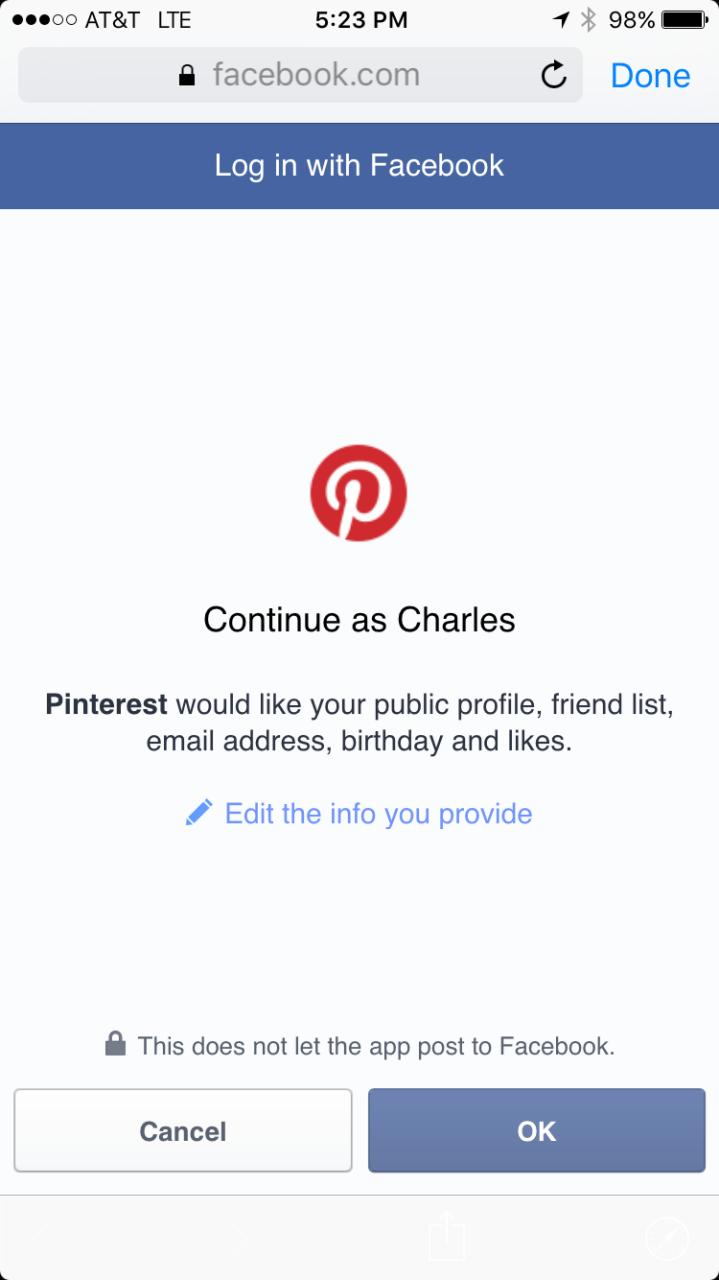
\includegraphics[scale=0.45]{chapters/images/chp2/desktopaccess1.jpg}
    \caption{A classic user consent on Facebook}
    \label{fig:usercon1}
\end{figure}

A first draft of the flowchart sequence is presented in Fig.~\ref{fig:flow1}. The simple steps are:

\begin{enumerate}
    \item The user asks App to suggest contacts.
    \item App says that to be done it needs the authorization here.
    \item App sends the user to Facebook. Here, Facebook asks him directly for authorization for App to access his friend list on his behalf. It does this by presenting the user consent form, which he can either accept or not. Let's assume he accepts.
    \item Facebook happily obliges, giving App the user's friend list. App then uses this information to tailor suggested contacts for him.
\end{enumerate}

However, it is necessary to specifically deal with the distinction of the two grant types in order to better integrate our concepts into a final flowchart.

\subsection{Trusted/Untrusted clients}

In \textit{\oauth} there are only two levels of trust: \textbf{confidential} and \textbf{public}. 
Therefore, a client could be categorized into either of this trust levels following the two simple capabilities of storing and transmitting information securely.

A \textit{trusted client} (\textbf{confidential}) is an application capable of storing and transmitting securely information (credentials, tokens, any other resources necessary for their application).
For example, it could be a 3-tier client-server-DBMS application where the back-end guarantees secure storage and transmission actions for confidential information. 

Instead, an \textit{untrusted client} (\textbf{public}) is one which is incapable of doing such things and so they cannot be trusted on storing/transmitting securely the needed data. All browser-based applications are untrusted clients (HTML/JS) because all the confidential data should be stored in the browser that is absolutely accessible by everyone.
It must be underlined that both capabilities of storing and transmitting must be fulfilled in order to call a client \textit{trusted}.

When the user accepts this form, he has agreed to allow App to access to his Facebook friend list on his behalf. In simple terms, the user has delegated read-only authority to App for his Facebook friend list.
This workflow can be curated some more. There is a very important step in the
preceding process that requires a larger discussion. It is step 4 where App and
Facebook finally exchange the information that has been requested. In the previous diagram, it has been presented as a single step where Facebook gives the information to App. However, in reality, this is a much more complicated exchange that occurs, which depends on many factors. Since this secure and controlled exchange of information is at the crux of what \oauth\ does, it is better to take a closer look.

\begin{figure}
    \centering
    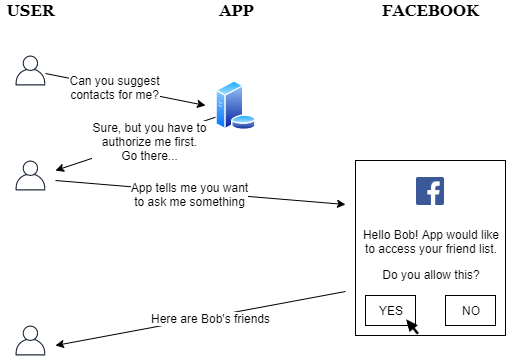
\includegraphics[scale=0.74]{chapters/images/chp2/flow1.png}
    \caption{First draft of the flow}
    \label{fig:flow1}
    \vspace{0.5cm}
\end{figure}

\vspace{1cm}

\section{Token and endpoints management}
Token and endpoints are two important keywords of \textit{\oauth}. In particular, a \textit{token} is an abstraction that replaces that classic \textit{username} and \textit{password} with a single identifier that might have different formats, structures and methods of utilization based on the server that implements it.

Instead, the \textit{endpoints} are crucial for the protocol. In Section 3 of the \rfc{6749}\ specification \cite{RFC6749}, \textit{\oauth} defines three endpoints:

\begin{itemize}
    \item Authorization endpoint
    \item Token endpoint
    \item Redirection endpoint
\end{itemize}

Obviously, not every grant types defines the first two ones.

\subsection{Access and refresh token}
\label{accref}
In \textit{\oauth} two types of token are distinguished.

\textbf{Access token}, that is a very long string that represents the authorization given to the client.

\textbf{Refresh token}, a particular family of tokens used to retrieve a new access token when the current one becomes invalid or expires. They are different from the classic ones because intended to be consumed only with \textit{AuthZ} servers (not resource servers). In Fig.~\ref{fig:refreshtok} we can see an example of how the refresh token is used when the access one expires.



\begin{figure}
    \centering
    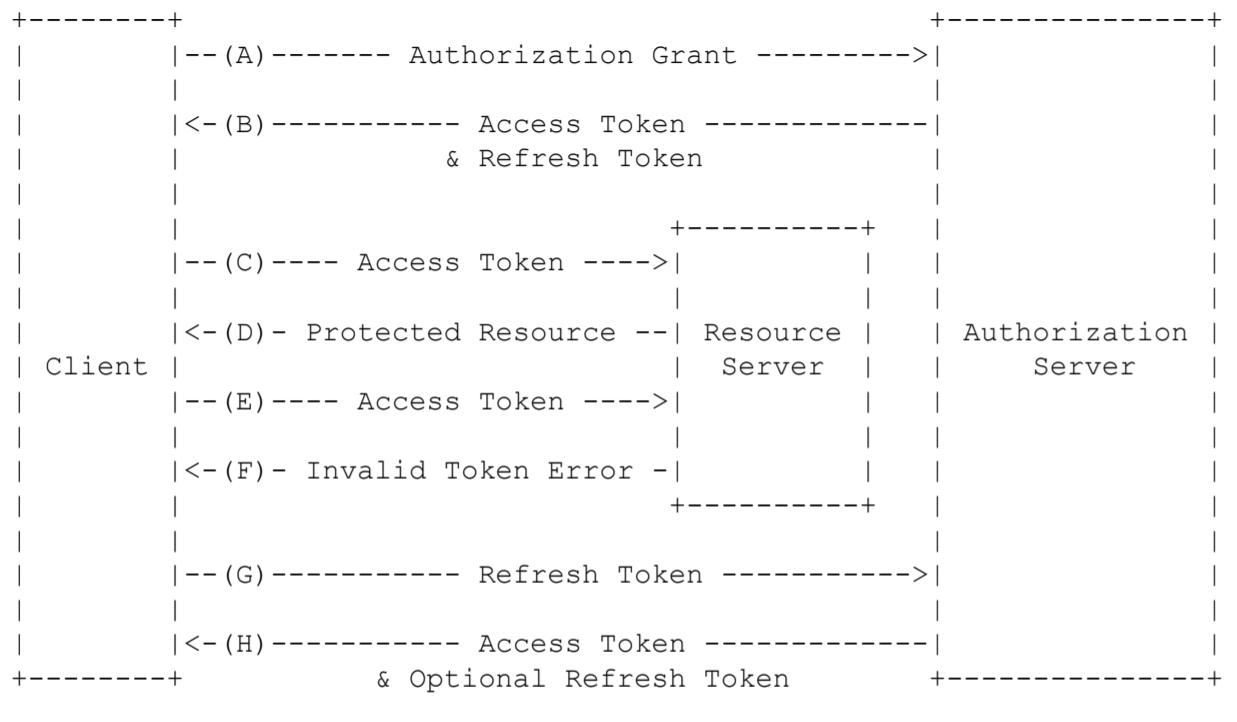
\includegraphics[scale=0.5]{chapters/images/chp2/tokenref.jpg}
    \caption{\rfc{6749} refresh token usage}
    \label{fig:refreshtok}
\end{figure}

\vspace{1cm}

\subsection{Authorization and token endpoints}
The \textbf{authorization endpoint} is used by the client to obtain authorization from the resource owner via user-agent redirection (the authorization server must first verify the identity of the resource owner, e.g. using OIDC) and it must use TLS\footnote{Transport Layer Security, "[...] cryptographic protocols designed to provide communications security over a computer network.". Source: \url{https://en.wikipedia.org/wiki/Transport_Layer_Security}} in order to have secure confidential data transmissions.

The \textbf{token endpoint} has the role of waiting for the client in order to return an access token in exchange of an authorization code or a refresh token. That kind of endpoint is not used in the implicit grant type (see section \ref{section22}), because in this case the token is issued directly.

\section{Client-side flow (untrusted)}
So far, the implicit grant flow is optimized for scripting language based clients. As a result of the resource owner authorization, the client is issued an access token directly without issuing an authorization code. This flow is defined in the Section 4.2 of the \rfc{6749}\ \cite{RFC6749}. It is important to say that, when using this flow, the authorization server does not authenticate the client (in some cases this could be done via the redirection URI). In the Fig.~\ref{fig:flowa} we can see the schema in detail. The steps from the specification are as follows:

\begin{itemize}
    \item[(A)]The client application initiates the flow by sending the user's user-agent to the appropriate authorization endpoint.
    \item[(B)]The authorization server of the service provider authenticates the resource owner and attempts to gain consent by presenting the user consent form.
    \item[(C)]If the user accepts consent, the AuthZ server redirects it to the client application using the redirection endpoint retrieved from the authorization request, including the access token in the URI.
    \item[(D)]The user-agent proceeds with the redirection, stripping the fragment and retaining the properties locally.
    \item[(E)]The client serves a web page that is capable of parsing the fragment and extracting the access token.
    \item[(F)]The user-agent extracts the access token using a script provided by the server.
    \item[(G)] At the end, the client will have the access token.
\end{itemize}

It must be noticed that (A) and (B) are split into two parts because they both pass through the \textit{user-agent}.

\begin{figure}[htbp]
    \centering
    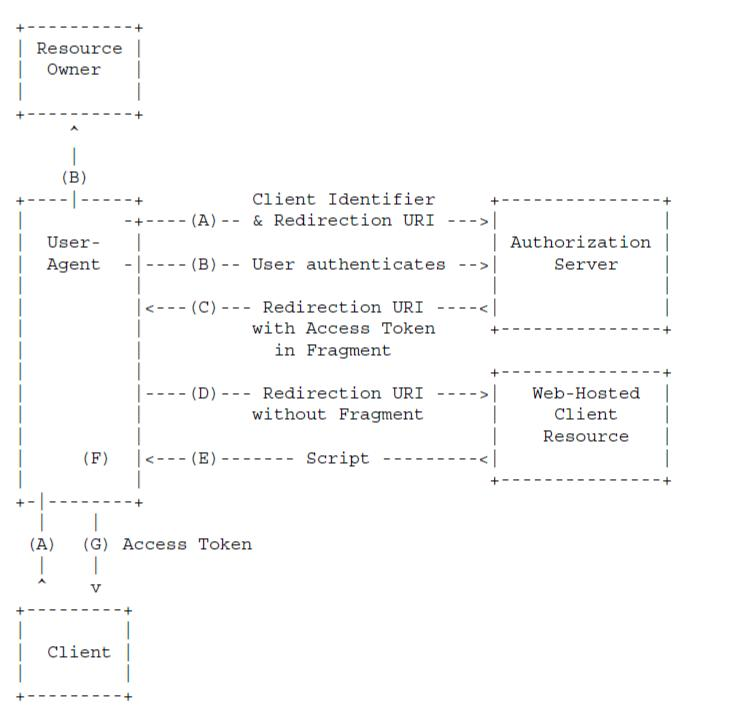
\includegraphics[scale=0.6]{chapters/images/chp2/client.jpg}
    \caption{\rfc{6749}\ implicit grant flow}
    \label{fig:flowa}
\end{figure}

\vspace{1cm}

\subsection{Analysis of exchanged messages}
At this point, it is clear that for what concerns the client-side implicit grant type we have only an \textbf{authorization request} and an \textbf{access token response}. Both of them must be encoded accordingly to the specification into the endpoint URI in the \textit{application/x-www-form-urlencoded} format.

\subsubsection{Authorization request}
\label{authreq}
The client MUST build this request using these parameters into the URI:

\texttt{response\_type}

\hspace{0.5cm}REQUIRED. The type has to be \textit{token}.

\texttt{client\_id}

\hspace{0.5cm}REQUIRED. This value must be set with the application's unique client ID.

\texttt{redirect\_uri}

\hspace{0.5cm}OPTIONAL. This value could be set with the URI of the redirection endpoint used by 

\hspace{0.5cm}the service provider to return the response, whether that is an access token in the case of

\hspace{0.5cm} a successful request, or an error message in the case of a failed request.

\texttt{scope}

\hspace{0.5cm}OPTIONAL. The scope of permissions that we are requesting on behalf of the user.

\vspace{0.5cm}

\texttt{state}

\hspace{0.5cm}RECOMMENDED. String issued by the client in order to maintain a state with the response.

\hspace{0.5cm}Value used by the AuthZ server to redirect the user-agent back to the client.

\hspace{0.5cm}As it will be shown in the following chapters, the param should be used to avoid CSRF\footnote{Cross-site request forgery, "[...] when a malicious program causes a user's web browser to perform an unwanted action on a trusted site on which the user is currently authenticated.". Source: \url{https://auth0.com/docs/protocols/oauth2/mitigate-csrf-attacks}}.

\subsubsection{Error response}
\label{tokenerr}
For many reasons could happen that the request is not accepted by the resource owner. In this case, an error message is built with those parameters in the fragment of the URI of redirection:

\texttt{error}

\hspace{0.5cm}REQUIRED. Single ASCII code representing the error:

\begin{itemize}
\item[] \begin{itemize}
        \item \texttt{invalid\_request}
        \item \texttt{unauthorized\_client}
        \item \texttt{access\_denied}
        \item \texttt{unsupported\_response\_type}
        \item \texttt{invalid\_scope}
        \item \texttt{server\_error}
        \item \texttt{temporarily\_unavailable}
\end{itemize}
\end{itemize}

\texttt{error\_description}

\hspace{0.5cm}OPTIONAL. Human-readable message describing what caused the error.

\texttt{error\_uri}

\hspace{0.5cm}OPTIONAL. Link to more information about the error.

\texttt{state}

\hspace{0.5cm}REQUIRED. If a state parameter was present in the request.

\subsubsection{Access token response}
When the provider (e.g. Facebook) grants the access request, according to the specification it sends a positive response adding to the fragment component of the redirection URI in the \textit{application/x-www-form-urlencoded} format the following parameters:

\texttt{access\_token}

\hspace{0.5cm}REQUIRED. It is this token value that we will eventually use to access

\hspace{0.5cm}the user's profile and feed data.

\texttt{token\_type}

\hspace{0.5cm}REQUIRED. As it suggests, specifies the type of token used

\hspace{0.5cm}to make a protected resource request.

\texttt{expires\_in}

\hspace{0.5cm}RECOMMENDED. The lifetime of the token in seconds. It could not be returned by the server.

\texttt{scope}

\hspace{0.5cm}REQUIRED. The scopes of the access token.

\hspace{0.5cm}OPTIONAL. If they are the same requested by the client.

\texttt{state}

\hspace{0.5cm}REQUIRED. If a state parameter was present in the request.

\section{Server-side flow (trusted)}
\label{authcg}

The AuthZ code grant is used to retrieve access tokens and (OPTIONAL) refresh tokens and it is built for client confidentiality. The AuthZ code is delivered by using an AuthZ server as a broker between client and resource owner. The server authenticates the owner of the resources and obtains authorization before directing it back to the client with the AuthZ code. This flow is described in Section 4.1 of the \rfc{6749}\ \cite{RFC6749}. It is important to point out that, for this flow, the resource owner only authenticates with the authorization server, providing a few important security benefits that will be discussed later on (e.g. client authentication and secure transmission). In Fig.~\ref{fig:serverflow} it is provided a detailed description of this flow:

\begin{itemize}
    \item[(A)]The client application initiates the flow by sending the user's user-agent to the appropriate authorization endpoint.
    \item[(B)]The authentication server of the service provider authenticates the resource owner and attempts to gain consent by presenting the user consent form.
    \item[(C)] The AuthZ server redirects the user back to the client application via the redirection endpoint provided in the authorization request (after that the user has given consent). The redirection endpoint's URI will include the Authz code and the state provided by the client.
    \item[(D)]Using the retrieved authorization token, the client requests the access token from the appropriate endpoint. Simultaneously, the client also has to authenticate using its credentials in the same request.
    \item[(E)] The service provider checks for the authentication, authorization and the redirection URI of step (C). Finally, in case of positive acknowledgement, an access token is issued (possibly, a refresh token too, depending on the server implementation).
\end{itemize}

It must be noticed that, with respect to the implicit grant flow, in addition to the steps (A) and (B), now step (C) too is divided because it passes through the \textit{user-agent}.



\vspace{0.5cm}

\begin{figure}[htbp]
    \centering
    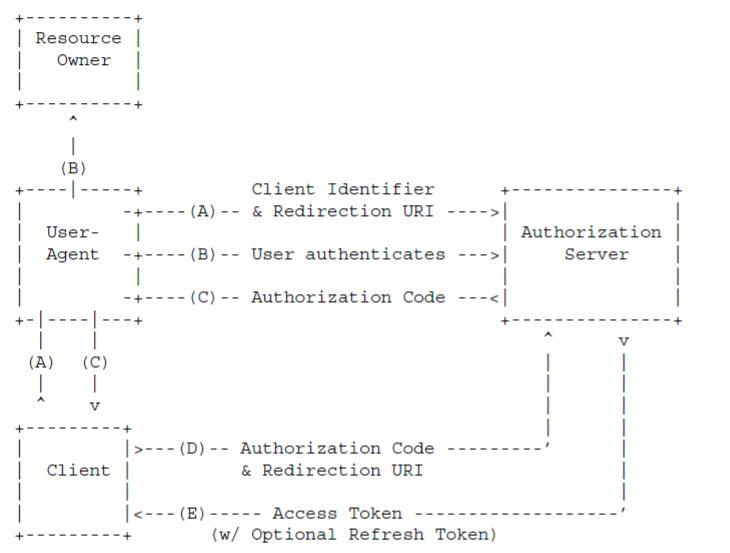
\includegraphics[scale=0.7]{chapters/images/chp2/server.jpg}
    \caption{\rfc{6749}\ authorization code grant}
    \label{fig:serverflow}
\end{figure}

\vspace{1cm}

\subsection{Analysis of exchanged messages}
The exchanged messages flow is more complex now. Throughout the AuthZ Code Grant flow, two more messages that precede the token request and response are added: the \textbf{authorization request} and the \textbf{authorization response}. Furthermore, it must be implemented the \textit{token refresh} usage (that still it is not always returned by the authorization server). However, here every message must be encoded according to the specification into the URI too using the \textit{application/x-www-form-urlencoded} format.

\subsubsection{Authorization request}

According to the specification, this request is the one to gain consent from the user. This message is nearly identical to the authorization request we made in the previous section for the implicit grant flow (\ref{authreq}), except for one important difference: the value of the \texttt{response\_type} parameter MUST be set to \textit{code} instead of \textit{token}.

\subsubsection{Authorization response}
If the request URL is correctly formatted and constructed, the resource owner will send back a response. If the response will be positive, an authorization code is sent in order to be afterwards converted in an access token.
The possible parameters that can be expected in the preceding response are now in the query component and not in the fragment one:

\texttt{code}

\hspace{0.5cm}REQUIRED. AuthZ code to be exchanged.

\texttt{state}

\hspace{0.5cm}REQUIRED. If a state parameter was present in the request.

\vspace{0.5cm}

On the other hand, if the response will be negative, the error will be structured as in the implicit grant flow (same properties as in \ref{tokenerr}). The difference relies only in the fact that it is returned in the query component instead of the fragment one.


\subsubsection{Token request}
Once that the authorization code has been retrieved, it can be used to exchange an access token. With this objective, the client makes a request by using a \textit{POST}, specifying in the body section the following parameters:

\texttt{grant\_type}

\hspace{0.5cm}REQUIRED. The value MUST be "authorization\_code".

\texttt{code}

\hspace{0.5cm}REQUIRED. It MUST be set to the value of the previously retrieved

\hspace{0.5cm}authorization code

\texttt{redirect\_uri}

\hspace{0.5cm}REQUIRED. If a redirect\_uri parameter was present in the request.

\texttt{client\_id}

\hspace{0.5cm}REQUIRED. The application unique Client ID.

\vspace{0.5cm}

Additionally,in order to pass these parameters to the access token request, the client
application must also identify itself with the service provider. This is an added
layer of security (only necessary for trusted clients) and it is known as \textit{client
authentication}.
It entails the secure transmission of the client credentials to the service provider for validation. It must be pointed out that although the \oauth\ specification doesn't specify any particular authentication scheme for client authentication, this is typically done using HTTP basic authentication [RFC-2617].
In other words, it is the Base64-encoded value of the client credentials in
the form:

\hspace{0.5cm}\texttt{[CLIENT\_ID]:[CLIENT\_SECRET]}

\subsubsection{Token response}
As it has been encountered in the previous responses, if the authorization code is valid, we will get our token or an error otherwise. Depending on the implemented server, we could possibly get an optional refresh token (\ref{accref}) in order to update our expired token without doing all the previous steps.

For a \textbf{success} response it is sent back a message with the following parameters in the entity-body (e.g.in JSON):

\texttt{access\_token}

\hspace{0.5cm}REQUIRED. It contains the token: successful authorization and access token request! 

\texttt{token\_type}

\hspace{0.5cm}REQUIRED. Defines the type of token sent.

\hspace{0.5cm}In almost all of the cases this will be \textit{bearer}.

\texttt{expires\_in}

\hspace{0.5cm}RECOMMENDED. The time-to-live of the token.

\hspace{0.5cm}If this value is 7200, that means that the access token will expire

\hspace{0.5cm}two hours from the time the response message was generated.

\vspace{0.5cm}

\texttt{refresh\_token}

\hspace{0.5cm}OPTIONAL. It may be used to refresh the access token in case it expires.

\texttt{scope}

\hspace{0.5cm}REQUIRED. The authorized scopes of the access token.

\hspace{0.5cm}OPTIONAL. If they are the same requested by the client.

\vspace{0.5cm}


\section{About mobile applications}
Typically, when someone talks about \textit{mobile application}, he is referring to one of the two types of applications:

\begin{itemize}
    \item Mobile-optimized web application
    \item Native mobile application
\end{itemize}

The first one is nothing more than a customized browser that runs the web app optimized for the small screen. Since that, the same rules as a desktop web browser are applied.
The second one though, is a natively installed mobile app, an entirely new platform developed in recent years. For this last type, what flow should be used? 

In order to answer this question, just as developing other types of client apps, the flow to be used is based on whether the platform is suitable for being trusted or not. In order for a mobile application to be considered trusted, it must be able to securely store and transmit confidential information. This can really only be achieved in
one way, with the use of a back-end server. If a mobile application has a back-end server that powers it, this server can also be used to securely store and transmit any confidential information it needs to. In this case, yes, this particular type of mobile application can be considered trusted, and should therefore use the authorization code grant flow (as for a web application with a server). 

In the absence of it though, the application will be unable to securely store and transmit confidential information, and cannot be considered trusted. In this scenario, the mobile application should use the implicit grant flow (as for a standalone web app).


\subsection{Secure storage APIs}
It is quite common that not all mobile applications are powered by a back-end server. Rather than use the implicit grant flow, there is a solution that can still archive secure (not strictly) storage capabilities by exploiting secure storage APIs in some mobile platforms like iOS and Android.  For the most part, this is enough for most applications to be considered trusted. Client credentials can be stored here and they can communicate directly with the service provider through the application, accessing these secrets via the APIs without the use of a back-end server.

However, strictly speaking, this is not considered trusted. It is true that the confidential data is encrypted, but it is accessible by the attacker. Data and user/attacker are in the same \textit{space} using this method, while with a back-end server the so called user/attacker space is external with respect to the storage services and not accessible. The platform's secure storage APIs may well be extremely secure and difficult for attackers to break, but in strict terms it is possible and, in the world of security, \textit{possible} should be assumed as \textit{probable}. This is why mobile applications that do not have back-end servers, but make use of the mobile platform's secure storage APIs, should not be considered trusted and should therefore not use the authorization code grant flow.

Since the architecture of the mobile application can be flexible, there is no reason why the application has to use a single authorization workflow. Given a mobile application and a back-end server, it is possible to create a hybrid architecture to leverage the best of both worlds.
    
    \chapter{Advantages and disadvantages}
Since in the previous chapters the majority of advantages and disadvantages of the protocol have been already discussed, in this chapter we complete our \textit{OAuth2} description by showing a complete work flow comparison (taking into account other flows defined by the protocol but not so used nowadays) and a brief introduction on the extensions in order to better understand its peculiarities. 

\minitoc
\section{Secondary flows comparison}
Until now, all the practical aspects of the standard RFC-6749 \cite{RFC6749} have been analyzed, but not all the defined ones. In particular, there are two other types of work flows in the specification: \textit{Resource Owner Password Credentials Grant} and \textit{Client Credentials Grant}. These two flows are not frequently used, but they can be helpful in some particular cases.

\subsection{Resource Owner Password Credentials Grant}
Described in Section 4.3 of the specification, this flow operates by using the user's actual credentials to gain an access token. It is not the best in terms of security. This goes against the other grant types, where the client application is completely unaware of the user's credentials. However, in this grant type, users send their credentials to the client application that, on their behalf, uses those credentials to access protected resources.
Once the client application has a user's credentials, it uses them to gain an access token, just as in the other grant types. In this sense, risk is slightly mitigated, compared to using the credentials directly, since tokens have limited scope and duration (unlike passwords). However, the passing and delegation of user credentials is highly undesirable due to the risk of leaking this important information.

Nevertheless, it could be useful when neither of the two others flows are available (implicit grant and authorization code grant).

\subsection{Client Credentials Grant}
Described in Section 4.4 of the RFC-6749, this type of flow is slightly different from the others. While the first three of them request access tokens on behalf of a user, this last one request access tokens on behalf of the client application. There may be occasions where the client application has resources with a service provider that are owned and consumed by the client application itself, and not by an end-user. For instance, a client application that uses Amazon RDS\footnote{Amazon Relational Database Service, "[...] makes it easy to set up, operate, and scale a relational database in the cloud. It provides cost-efficient and resizable capacity while automating time-consuming administration tasks such as hardware provisioning [..]". Source: \url{https://aws.amazon.com/rds/}} to persist its own application data (as opposed to a user's data). In this case, this grant is preferred. With this workflow, the client application can request an access token on its own behalf and then use that access token to access the protected resources it needs. The good news are that no user intervention is required and no additional risk is exposed.

\section{OAuth2 extensions}
Extensions are an ample, sophisticated and important key concept of the OAuth2 protocol. Indeed, they do not fall into the same specification and more or less everyone of them has its own RFC.

The implicit and the authorization code grant flows represent the majority of flows that application developers use. However, it is only a limited view with respect to the larger range of capabilities allowed by the framework. There are many extensions that can be added to the Open Authorization Framework to facilitate many additional use cases, but surely the most important ones are \textit{token types}, \textit{custom grant types} and \textit{OpenID Connect}.

\subsection{Token types}
Once a grant type is decided, the client application will interact with a service provider through the exchange of tokens. Once the user authenticates and authorizes the application, they are given a bearer token [RFC-6750], which the application can then use to access a protected resource on his behalf. The properties of these tokens are quite loosely defined, described by the specification simply as opaque string values that encapsulate an authentication for a particular user. They can simply be unique strings that match up with a set of permissions for a user. Many service providers implement their tokens in this non-standard, custom way. However, it is useful to know that there are two popular token formats that can be used by service providers, if desired:

\begin{itemize}
    \item JSON Web Tokens (JWT), described in RFC-7519 \cite{RFC7519}
    \item SAML assertions, described in RFC-7522
\end{itemize}

Both of these token formats describe a standard for the creation and usage of security tokens. These tokens are known as security tokens, because they make use of cryptography to facilitate features that would not normally be allowed via simple opaque string values.

JWTs are most commonly seen in the consumer space (they are used in the OpenID Connect protocol). Compared with SAML assertions, JWTs can be considered a simpler version of security token than a SAML assertion, with a simpler format and encoding syntax. SAML assertions, on the other hand, employ a standard for security tokens that is more expressive and powerful than JWTs, at the expense of added complexity. These will typically be seen in the enterprise space where SAML integration for authentication is more prevalent. Both of these formats can act as bearer tokens in the OAuth 2.0 protocol, as long as they are supported by the service provider.


\subsection{Custom grant types}
When the client application interacts with a service provider, such as Facebook, it does so by using a particular, predefined grant type. Previously, they have been discussed the two most commonly used grant types:

\begin{itemize}
    \item Authorization code grant
    \item Implicit grant
\end{itemize}

\noindent And the two additional grant types that are supported:

\begin{itemize}
    \item Resource owner password credentials grant
    \item Client credentials grant
\end{itemize}

\noindent They, as it has already been explained, are less commonly supported by consumer service providers, such as Google and Facebook. However, it must be pointed out that in addition to natively supporting these four grant types, the \textit{OAuth 2.0} framework allows for the specification of additional custom grant types. These will be determined and implemented by the service provider. So, perhaps a workplace decides to use \textit{OAuth 2.0} to restrict access to certain parts of the company's data, but the IT team and security team do not want to use any of the four natively supported grant flows. They can, instead, design and implement their own grant type, which the client application will subsequently use to request access tokens and access those protected resources.

\subsection{Authorization backend}
One of the major benefits of the OAuth 2.0 protocol is that it has the ability to encapsulate and abstract away the authentication layer of a service, wrapping it with a standard, uniform layer for client applications to consume. For instance, a company may be using a Kerberos-based authentication system (e.g. LDAP [RFC-4511]), for the company's internal authentication. They may, at some point, choose to wrap this with an OAuth 2.0 layer, which would effectively encapsulate their authentication layer and present a uniform interface to any interested parties. Now, they can change their internal authentication methodologies, say, to SAML, and clients would be largely unaware of that (they may be presented a different user consent screen, but other than that, behavior should be unaffected). This is a very powerful concept. Abstracting away the authentication layer provides a uniform interface for clients while maintaining flexibility for the underlying protocols to change without affecting (that is, breaking) clients.

\subsubsection{OpenID Connect}
The framework describes a protocol for managing authorization to protected resources for a service. It does not, however, describe methods for authentication. \textit{OpenID Connect} \cite{openid} is a protocol built on top of \textit{OAuth2} in order to provide a complete solution for both authentication and authorization. As showed in Fig.~\ref{fig:oidc}, OIDC provides an identity layer on top of the authorization protocol described by OAuth2. It allows clients to check the identity of an end-user when it authenticates in order to  authorize the OAuth2 consent. Most importantly, this can all be done by the client application without having to store or manage passwords.

\begin{figure}
    \centering
    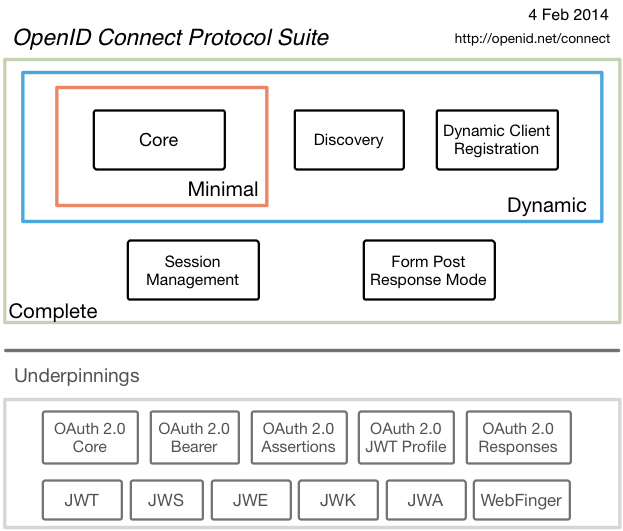
\includegraphics[scale=2.0]{chapters/images/chp3/OpenIDC-map.png}
    \caption[caption]{OpenID Connect protocol suite\\\hspace{\textwidth}Source:\hspace{0.2cm}\url{https://openid.net/connect/}}
    \label{fig:oidc}
\end{figure}

Previously, the concepts of \textbf{federated identity} and \textbf{delegated authority} have been introduced and it has been mentioned that they are actually the same underlying concept. In one delegated authority scenario, the user delegates authority for a client application to access some protected resource on their behalf, say, access to their Facebook friend list. However, this protected resource could be anything. It could even be their profile information as stored by Facebook. Delegating access to this resource gives the client application the means of verifying the end-user's identity without ever seeing their credentials. As an example, it is interesting how this is accomplished with OpenID Connect using a familiar OAuth 2.0 workflow. What follows is a modified version of the authorization code grant flow that we explored previously:

\begin{itemize}
    \item[1.] The client application initiates the authorization request using the authorization code grant flow. However, in this authorization request, a subset of the following OpenID Connect scopes is requested:
    \item[] \begin{itemize}
        \item \texttt{openid}: REQUIRED. It means that the client is making an OIDC request
        \item \texttt{profile}: OPTIONAL. This requests access to the user's
    profile information
        \item \texttt{email}: OPTIONAL. This requests access to the user's e-mail address
        \item \texttt{address}: OPTIONAL. This requests access to the user's  address information
        \item \texttt{phone}: OPTIONAL. This requests access to the user's phone number
    \end{itemize}
    
    \item[2.] Here the server must validate the parameters. In particular, OIDC defines more OPTIONAL params (e.g. \texttt{nonce}, \texttt{prompt} and so on) that are essential to manage the authentication (e.g. rather than the authentication itself, whether the user is already authenticated or not). After that the server validates the parameters, if it is a valid request for login, the user is presented with the same user consent screen that we are familiar with, with the difference that it MAY be specified that the user authorizes the relying party (client) to authenticate it. If it accepts, it will be redirected back to the client application via the redirection endpoint, passing along with it the corresponding authorization code (as OAuth2 requires).
    \item[3.] The client application will take this authorization code and make a request to the service provider's token endpoint to exchange it for an access token. The server must know that the corresponding AuthZ code was issued from a OIDC authentication request and must check the client\_id correspondence of it. It builds up the \texttt{id\_token} that is a JWT which contains private claims about the authenticated user (\texttt{name}, \texttt{address} and so on) and other claims defined in the Section 4.1 of the RFC-7519 \cite{RFC7519} (such as \texttt{iss} that represents the issuer and \texttt{sub} that represents a unique identifier of the authenticated user).
    \item[4.] The response from this request will contain an access token (as the property \texttt{access\_token}). However, it will contain the additional token known as an \textit{ID token} (as the property \texttt{id\_token}). The client MUST decrypt the token by using the specified cryptographic operations contained in the JOSE Header (Section 5 of RFC-7519), validate the JWT ID Token and retrieve the claims about the user, the issuer and so on, in order to ensure the truthfulness of the message response. Finally, the user identity provided by the AuthZ server using OIDC on top of OAuth2 is verified.
\end{itemize}


As it can be seen, this flow is very similar to the authorization code grant flow that has been discussed earlier, except now it is possible to verify the identity of the user by consuming the ID token built and signed by the AuthZ server, something that was not possible to do with OAuth 2.0 alone. It is an elegant solution for providing a full end-to-end authentication and authorization framework.
    
    \chapter{Residual risks}
In this last chapter are presented some important best practices along with a deep analysis of the common attacks on \textit{OAuth2}. All the risks linked to the protocol are described in the Section 10 of the RFC-6749 \cite{RFC6749}.

\minitoc

\section{Introduction}
Just as with any application, security should be a top priority. This is especially true for applications that utilize this protocol. In order to understand why it is true, could be helpful to summarize what OAuth2 does. Recalling that, it has been discussed how OAuth2 provides federated identity as well as delegated authority. If there is no diligence with security practices during the implementation, some very dangerous holes can be exposed for attackers to exploit.
Indeed, when dealing with federated identity and delegated authority (since these are very powerful practices that can provide attackers with a lot of power) the developers must be extra vigilant.

If an attacker were somehow able to exploit an application to game either of these concepts, they may be able to do the following:

\begin{itemize}
    \item Impersonate users
    \item Impersonate client applications
    \item Grant themselves otherwise unauthorized permissions
    \item Gain access to protected data and resources
\end{itemize}

In order to fight this, there must be extra carefulness with the implementation with regard to the client integration with the service provider via OAuth2. 

\section{Best practices}
There are surely countless ways that a given application can be exploited. The objective is to minimize the attack vectors available to attackers, but it is not possible to cover all the possibilities. What follows is a non-exhaustive list of security best practices that will help to keep an application as secure as possible. 

\subsubsection{Use the authorization code grant flow}
The authorization code grant flow is by far the most secure flow available. It utilizes a back-end server to securely store and transmit sensitive properties, such as client credentials and tokens, to and from the service provider.
Proper use of a server to facilitate these communications will completely abstract, and hide, the flows from the end-user, as well as any attackers.

\subsubsection{Use TLS}
It might seem like an obvious tip, but it is important enough to note. The use of secure communication channels applies for when the client application talks to service providers, as well as when the service providers talk to the client application. When a client application talks to the service provider, it does so by interacting with their authorization and token endpoints. It must be ensured that they utilize TLS so that the communication with them is secure and encrypted.

Additionally, when the service provider talks back to the client application, it does so via the redirect URI that has been previously passed to it. Even this endpoint, owned by the developer, must utilizes TLS as well.

\subsubsection{Use the refresh token}
For clients using the authorization code grant flow, depending on the service provider, a refresh token may be returned to the client. When an access token expires for a user, rather than requiring them to authenticate again, the refresh token can be used to request a new, valid access token. This is desirable from both a security standpoint as well as a usability standpoint.

In terms of security, the fewer times a user has to authenticate means the fewer times a user has to send their username and password across the Internet. This also means fewer opportunities for an attacker to steal them.

From a usability standpoint, this means that the application can function for longer periods of time without having to ask the users to re-log in.

\subsubsection{Use native browsers}
\label{native}
The use of native external browsers over embedded browsers pertains particularly to native applications (that is, desktop applications and mobile applications). Often, when implementing a native application, it can be chosen to initiate the authorization flow in either the native system browser or an embedded browser within the application.

For example, if someone is developing an iPhone application and wants to start the authorization flow for a user, he can choose to do this through the native iPhone Safari browser. Or, he can choose to use an embedded browser provided by the SDK directly in the application. This choice has many important, but subtle, consequences, relating to both security and usability. Initially, someone may wants to use an embedded browser for the application. This will provide a more seamless user experience since users can stay in the application without having to bring the native system browser to the front momentarily for authentication and authorization. However, there are some very good reasons to use the native system browser.

The most important reason for using the native system browser is that it can be leveraged the system Chrome to display security information related to the target service provider's authorization endpoint. For instance, native browsers will often display warnings for sites with invalid or expired certificates, whereas embedded browsers often do not. This makes phishing attacks easier.Native system browsers use a different cookie jar than embedded browsers. So, if a user already has an active session in the system browser, they can piggyback on this. Whereas, in an embedded browser, since sessions are not shared with the native browser, they will likely have to start a new session. Additionally, native system browsers may have plugins available to it, like password managers, which would not be available to embedded browsers.

\subsubsection{Do not use third-party scripts in the redirection endpoint}
When constructing a redirection endpoint, any third-party or externally loaded scripts must not be included, since they will have all sort of unauthorized accesses (URI, credentials and so on). It is possible that these scripts can be compromised and, if loaded externally, could leak the access tokens or authorization codes to attackers.
If the use of third-party scripts is essential, it must be ensured that those scripts execute first to both extract and remove the credentials from the URI before allowing any other scripts to execute.

The redirection endpoint has to contain scripts only to remove the credentials before redirecting the agent to another page, nothing else.

\subsubsection{Rotate the client credentials}
Just as it must be done with personal passwords, it should be a good practice to rotate the client credentials. This minimizes the attack vectors available to attackers since, if credentials are rotated regularly, they will have a more limited time to utilize them if they are leaked.
A good practice would be to rotate these credentials with every release (or major release, depending on the security requirements and development cycle).

\subsubsection{Request minimal scopes}
Recalling that a scope is simply a permission that the client application is requesting on behalf of the user, it is safer making sure that is requested only what is needed by the application, and no more. This may seem obvious, but as applications grow and evolve, their functionality changes with it. This may change the scope of the permissions that the application requires.

\subsubsection{When using the implicit grant flow, request read-only permissions}
As it has been discussed previously, clients that utilize the implicit grant flow are untrusted clients.
They are considered untrusted because they do not have a back-end server to facilitate secure communication with the service provider. So, when the service provider sends tokens to the client, it does so by attaching the token values to the URL fragment of the redirect URI. Because of this, those token values are available to the user and anyone else who has access to the user-agent. Additionally, the value may be cached in some access logs or browser history for an attacker to find.
Tokens granted to untrusted clients are inherently insecure for these reasons. Keeping this in mind, a good implementation should only request read-only permissions when utilizing the implicit grant flow from untrusted clients. This minimizes the risk in the case that a token gets leaked.


\subsubsection{Credentials and tokens out of reach of users}
The application's client credentials and the received tokens are sensitive properties. They must keep these as secure as possible, making sure not to expose them to users. It is assumed that, if a user can see them, an attacker can too. If an attacker can get hold of the application's client credentials, they can impersonate the client. If an attacker can get hold of a granted access token for a user, they can impersonate that user. It is best to keep these out of reach of the users entirely. This is best done by using a back-end server to store and transmit these values, never exposing them to the client.

\section{Common attacks analysis}
After some security best practices to keep the application secure, it is now time to take a look at some common attacks against \textit{OAuth2} clients that everyone should be aware of. Furthermore, they will also examined mitigation techniques that can be used to protect the application from such attacks.

\subsubsection{Cross-site request forgery}
\label{csrf}
CSRF is a powerful attack that has been gaining popularity with attackers in recent years. It involves tricking users into following a malicious link that performs an undesirable action on a trusted site without their knowledge, making use of their pre-existing sessions with that site.

For instance, we can imagine a user that has just logged into his bank in his favorite web browser. Now, in another tab, he opens an e-mail from a malicious user with a link that says "See cats here!" which leads to \texttt{http://www.catloversheaven.com/}.
This site is owned by the attacker and, while the user is browsing pictures, in the background, the website silently makes a call to \texttt{https://www.bank.com/transfer?to=373252 \\ 83\&amount=1000}.
Since the user already has a valid session with their bank, this request will be seen as valid. And so, while the user is enjoying the attacker-owned website, they have also unwittingly transferred \$1,000 out of their account and into the
attacker's account. This can be done in many ways: a malicious link that tricks victims into clicking, an \texttt{iframe} or \texttt{image} that automatically loads the malicious link, or even a redirection from an attacker-controlled page.

How is this relevant all of this to an OAuth2 client application? 
Reminding the first workflow with a typical authorization workflow previously discussed, it is possible to add another party (namely, the attacker). In this scenario (Fig.~\ref{fig:csrf}), the attacker sends a malicious authorization code or access token directly to the client application's redirect URI. Since the client application can't verify that the token is valid, it continues to use it to communicate with the service provider. As the token is attacker-owned, this may result in the attacker gaining access to the protected resources of the user.
This happens mainly because the client application has no way of verifying that the authorization code or access token that has been issued to it is the result of a valid request made by the application.

\vspace{1.5cm}

\begin{figure}[ht]
    \centering
    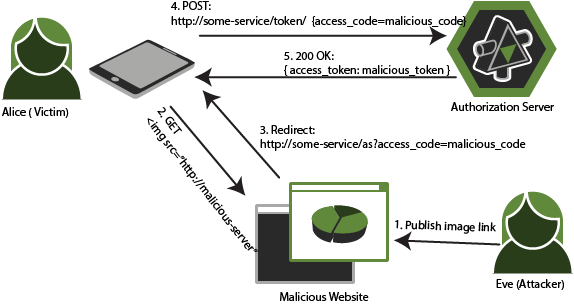
\includegraphics[scale=0.65]{chapters/images/chp4/csrf.png}
    \caption[CSRF on Oauth2]{CSRF on Oauth2.\\\hspace{\textwidth}Source:\hspace{0.2cm}\url{https://stackoverflow.com/a/42520213}}
    \label{fig:csrf}
\end{figure}

\vspace{1.5cm}

To avoid this attack, the client application must make use of the \texttt{state} param.
In order to protect the client application against CSRF, the developer must implement the ability to verify whether the authorization codes or access tokens issued to it are valid (that is, they are the result of a valid authorization request by the user from the client application). To do this, the client application must generate a session-specific, unguessable value that it can pass along with its authorization request. When an authorization code or access token is returned back to the redirect URI, the application can validate that value to ensure that it was indeed used as part of a valid authorization request initiated by the user, and not by some attacker.

If a \texttt{state} param value is passed to a service provider, the OAuth2 specification mandates that it MUST be returned back to the client application untouched. This mechanism is designed specifically to mitigate such CSRF attacks, and should be used particularly for this reason.

\subsubsection{Phishing}
Phishing is an attack in which an attacker creates a page or application that looks similar or identical to a target site with the intention that users will be unaware that it is a duplicate and so will enter secret information, like username and password, only to be captured by the impostor site.

OAuth2 client applications are vulnerable to phishing because they rely on sending a user's user-agent to and from the service provider endpoints in order to delegate authority. When developing the client application, everyone should consider the security implications of how the users will interact with the service provider to authenticate. A good rule of thumb is to follow the best practice mentioned earlier (see \ref{native}).

If native external browsers are used in an application, users will have an increased ability to verify the authenticity of the authorization endpoint that they are seeing.

\vspace{1cm}

\begin{figure}[ht]
    \centering
    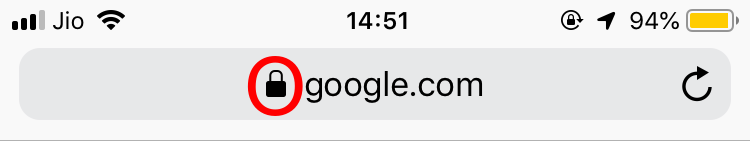
\includegraphics[scale=0.55]{chapters/images/chp4/oie_toIlpPOFRMdK.png}
    \caption{Example of site validity on Safari for iOS}
    \label{fig:ioslock}
\end{figure}

\vspace{0.5cm}

With native browsers, there are often more indicators of a site's validity (for example the lock next to the URL in iPhone's mobile Safari in Fig.~\ref{fig:ioslock}). This isn't the case with embedded browsers, which makes utilizing counterfeit pages much easier for attackers.

\subsubsection{Redirection URI manipulation}
When a client application makes an authorization request for a user, it passes along a \texttt{redirect\_uri} parameter. This parameter can be modified by an attacker, forcing the redirection to a third party URI.
Furthermore, if the application allows users to own or create a webspace of some sort that they control, like a homepage or a user profile page, they may be able to leverage it as part of their attack.

For example, considering the scenario where the application ExApp allows users to create a homepage on their domain. The user Eve may have a homepage that she controls at \texttt{www.exapp.com/users \\ /eve}. If the service provider (whith whom the app is interacting with) allows to register wildcard redirect URIs, like \texttt{www.exapp.com/\*}, or doesn't require to register a redirect URIs at all, then an attacker, such as Eve, would be able to use this homepage to her advantage.
What Eve could do is set up a fake link to log into the application, or even a counterfeit application entirely. When a user clicks on this link, they will be directed to the authorization endpoint of the service provider just as would be done from the real application. However, instead of passing the proper redirect URI, for example \texttt{www.exapp.com/callback}, this link passes her own malicious redirect URI which just happens to be her profile page, \texttt{www.goodapp.com/users/eve}. On this page, she can then intercept any authorization codes and access tokens, and proceed to impersonate users and access their protected resources.


\begin{figure}[ht]
    \centering
    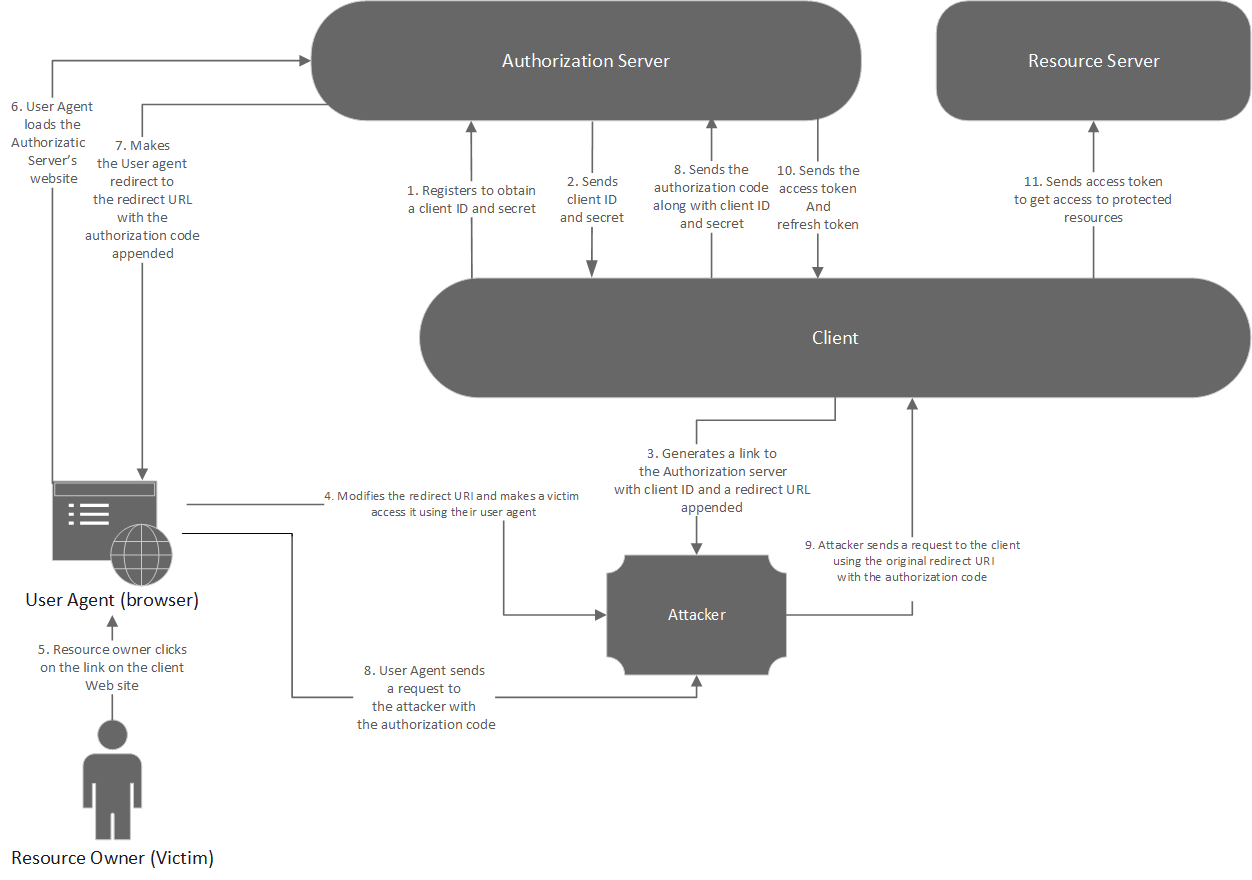
\includegraphics[scale=0.65]{chapters/images/chp4/authCodeURIAttack.png}
    \caption[Redirection URI manipulation's typical flow]{Redirection URI manipulation's typical flow.\\Source:\hspace{0.2cm}\url{https://www.thearmchaircritic.org}}
    \label{fig:reduri}
\end{figure}

It must be noticed that all Eve needs to do is convince a user to follow her malicious authorization link containing her attacker-controlled redirect URI. From the user's perspective, the user experience would be mostly the same since all that is different is the redirect URI (the attacker may choose to request additional scopes too).

To mitigate this, redirect URIs must be registered. If the service provider with whom the application is interacting with allows to register wildcard redirect URIs, they must be used sparingly. Furthermore, it should always choose to prefer to register fully-qualified redirect URIs over wildcard redirection endpoints. This is especially true if the service or application allows users to create a webspace that they control, like a homepage or profile page.

\subsubsection{Client and user impersonation}
A very basic attack that is often done is simple client or user impersonation.

In client impersonation, an attacker masquerades as the client application in order to gain access to the user's protected resources. This can be achieved quite simply if an attacker is able to get access to the client credentials (that is, the client ID and client secret). With this, they would be able to impersonate the client to the service provider and to end users.

In user impersonation, an attacker will masquerade as the end user. This can be done if an attacker is able to gain access to an issued access token. With this, they would be able to make requests to the service provider to access protected resources on behalf of the user, just as the application does.

To mitigate both of these attacks, the solution is simple: protect the client credentials, codes, and tokens from end users. If an attacker were able to see any of those, they would be granted the ability to impersonate the client application or the users, or both.



    
    % ------ APPENDIX A ------

\appendix
\chapter{User manual}
% ------ APPENDIX INTRO ------
This appendix explains how to correctly install and run the two implementations of the \oauth\ AuthZ Code Grant Flow: the former using as provider Google/Facebook and the latter using a custom AuthZ/Resource Server.
% ------ END OF APPENDIX INTRO ------

% ------ SECTION A.1 ------
\section{Software dependencies}
\label{appa}
Before installing and running the two implementations, there are some basic dependencies to install: \texttt{Docker} and \texttt{Docker-Compose}.

% ------ SECTION A.1.1 ------
\subsection{Docker}
\label{ublin}
The Docker Documentation \cite{docker} explains how to correctly install Docker on Windows/Ubuntu/macOS.

\paragraph{Ubuntu Linux (16.04 - 18.04 - 20.04)} First, all previous versions must be removed. 

\noindent From the bash terminal:
  
\texttt{\$ sudo apt-get remove docker docker-engine docker.io containerd runc}

\noindent Update and install packages to install dependencies over HTTPS:

\texttt{\$ sudo apt-get update}

\texttt{\$ sudo apt-get install apt-transport-https ca-certificates curl \textbackslash} \\
\indent \hspace{0.8cm} \texttt{gnupg-agent software-properties-common}

\noindent Add Docker’s official GPG key:

  \texttt{\$ curl -fsSL https://download.docker.com/linux/ubuntu/gpg | \textbackslash} \\
  \indent \hspace{0.8cm} \texttt{sudo apt-key add -}

\noindent Set-up the \textbf{stable} repository (change the \texttt{arch} param according to the architecture):

  \texttt{\$ sudo add-apt-repository \textbackslash} \\
  \indent \hspace{0.8cm} \texttt{"deb [arch=amd64] https://download.docker.com/linux/ubuntu \textbackslash} \\
  \indent \hspace{0.8cm} \texttt{\$(lsb\_release -cs) stable"}

\noindent Install Docker:

  \texttt{\$ sudo apt-get update}
  
  \texttt{\$ sudo apt-get install docker-ce docker-ce-cli containerd.io}

\noindent Add the current user to the \texttt{docker} group:
  
  \texttt{\$ sudo groupadd docker}
  
  \texttt{\$ sudo usermod -aG docker \$USER}

\noindent For different Linux distros or architectures, the Official Docs\footnote{\url{https://docs.docker.com/engine/install/}} is available.

\paragraph{Windows 10 Pro/Enterprise ($\geq Build 15063$)} The steps to follows are pretty straightforward:

\begin{itemize}
    \item[1.] Download Docker Desktop from the download page\footnote{\url{https://hub.docker.com/editions/community/docker-ce-desktop-windows/}}.
    \item[2.] Ensures that Hyper-V is enabled\footnote{\url{https://docs.microsoft.com/en-us/virtualization/hyper-v-on-windows/quick-start/enable-hyper-v}}.
    \item[3.] Double-click on the installer downloaded.
    \item[4.] Follow the standard installation procedure.
\end{itemize}

\paragraph{macOS ($\geq 10.13$)} Similarly to Windows:

\begin{itemize}
    \item[1.] Download Docker Desktop from the download page\footnote{\url{https://hub.docker.com/editions/community/docker-ce-desktop-mac/}}.
    \item[2.] Double-click on the \texttt{.img} downloaded.
    \item[3.] Drag the application in the Application folder.
\end{itemize}
% ------ END OF SECTION A.1.1 ------

% ------ SECTION A.1.2 ------
\subsection{Docker-Compose}
For Windows and macOS systems, \texttt{docker-compose} is included in the Docker Desktop installation.\\
On Ubuntu Linux, the steps follow.

\noindent Install PIP:

  \texttt{\$ sudo apt update}
  
  \texttt{\$ sudo apt install python3-pip}

\noindent Upgrade PIP:

  \texttt{\$ sudo pip3 install -U pip}

\noindent Install docker-compose:
  
  \texttt{\$ sudo pip3 install docker-compose}


% ------ END OF SECTION A.1.2 ------
% ------ END OF SECTION A.1 ------

% ------ SECTION A.2 ------
\section{Installation and use}
Once that \texttt{docker} and \texttt{docker-compose} are installed, the demos installation and use is not OS-dependent. Indeed, Docker Desktop (Windows/macOS) needs to be started as application first.

% ------ SECTION A.2.1 ------
\subsection{\oauth\ with Google/Facebook}
In order to install and run the implementation example that interacts with Google/Facebook, the file \texttt{docker-compose.yaml}\footnote{\url{https://github.com/nopesir/oauth-hw-security/releases}} is available in the resources as well as on GitHub as shown in Fig.~\ref{fig:rel1} (there are other files, but we only need the \texttt{.yaml} file).

\begin{figure}[h!]
    \centering
    \fbox{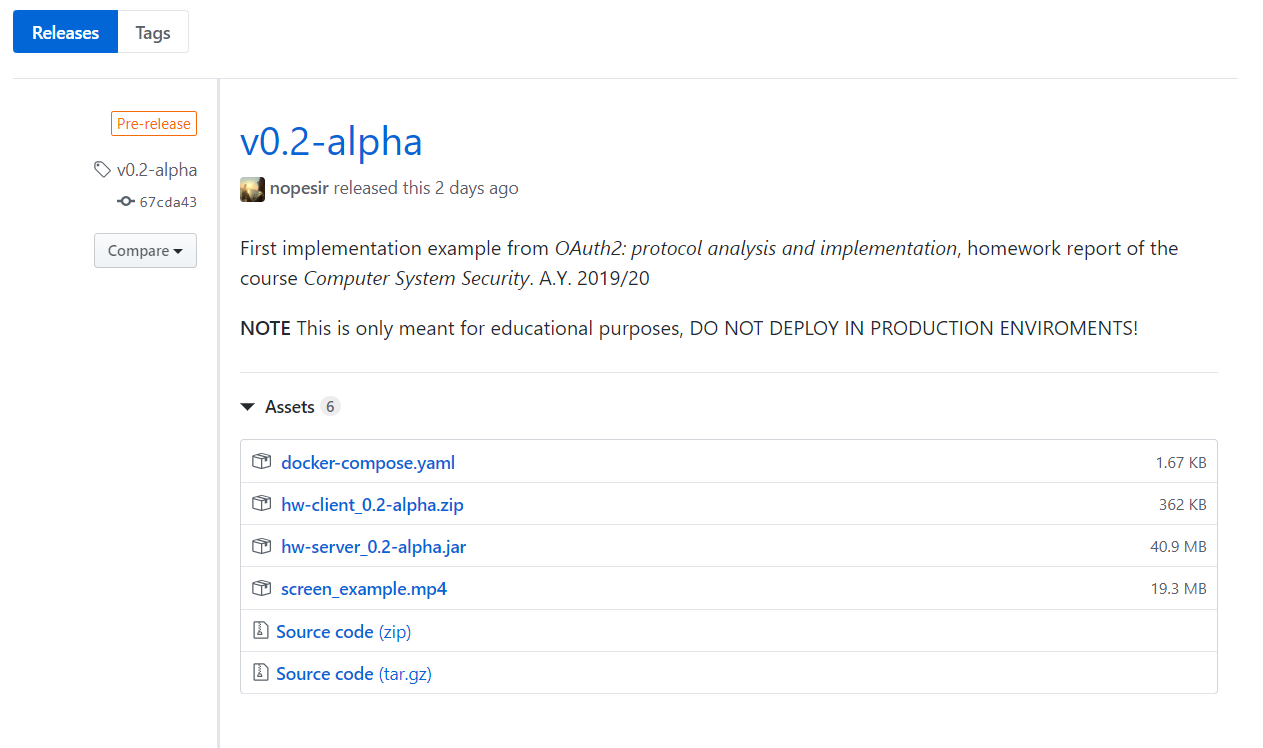
\includegraphics[scale=0.55]{chapters/images/chp5/release1.png}}
    \caption{GitHub Releases page: where to download the \texttt{docker-compose.yaml} file}
    \label{fig:rel1}
\end{figure}

\newpage

\noindent Then, in the same folder where \texttt{docker-compose.yaml} is, from the terminal:

  \texttt{\$ docker-compose up}

\noindent If all the dependencies are correctly installed and the docker daemon is running, \texttt{docker-compose} will automatically pull the containers, create the network namespace and start everything. The first run needs some time to download, but the next ones will use the downloaded data and will boot up the containers in a few seconds. The application now is running. From the browser, visit \texttt{http://localhost:9090} and the homepage will be displayed (Fig.~\ref{fig:home1}).

\begin{figure}[h!]
    \centering
    \fbox{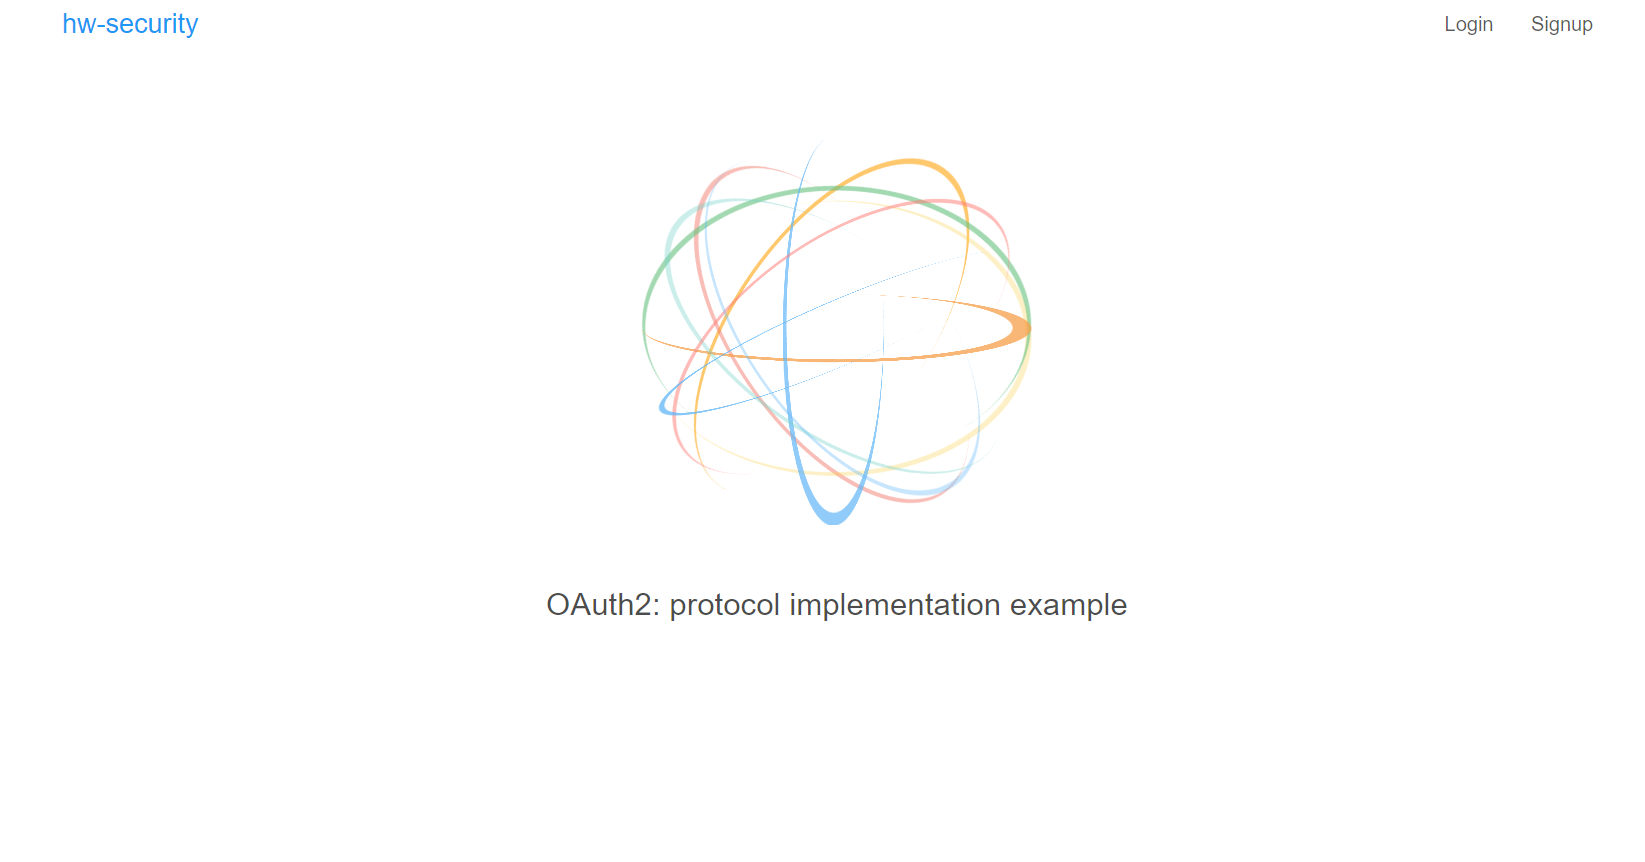
\includegraphics[scale=0.48]{chapters/images/chp5/screen1.png}}
    
    \caption{The homepage of the first implementation example}
    \label{fig:home1}
\end{figure}

\noindent To stop the application and safely detach all the resources, \texttt{Crtl+C} command on the terminal and finally a:

  \texttt{\$ docker-compose down}

\noindent The full screen video captioning of the example is available in the resources and in the Assets of the releases page\footnote{\scriptsize{\url{https://github.com/nopesir/oauth-hw-security/releases/download/v0.2-alpha/hw-security-screen.mp4}}}. 

\subsubsection{Troubleshooting}
\begin{itemize}
    \item Ensure to have ports \texttt{9090/tcp}, \texttt{8080/tcp} and \texttt{3306/tcp} available.
    \item Facebook login could give an error: Facebook App in test mode are accessible with \oauth\ only by the developer Facebook account\footnote{\url{https://developers.facebook.com/docs/apps/managing-development-cycle/\#step1}}, thus some test users must be added to the Facebook Developer's page. Use Google instead.
    \item Ensure to have at least 8GB of RAM on the machine.
    \item (Windows/macOS) Ensure that the Docker Desktop program is started.
    \item (Ubuntu Linux) Ensure that the Docker deamon is running.
\end{itemize}
% ------ END OF SECTION A.2.1 ------

% ------ SECTION A.2.2 ------
\subsection{\oauth\ with custom AuthZ/Resource servers}
In order to install and run the second example, the steps are almost the same as the previous subsection. The new \texttt{docker-compose.yaml} is available on the releases page\footnote{\url{https://github.com/nopesir/oauth-hw-security-custom/releases}} or in the resources (remove the previous \texttt{.yaml} file or choose another folder).

\noindent Then, in the same folder where \texttt{docker-compose.yaml} is, from the terminal:

  \texttt{\$ docker-compose up}

\noindent If all the dependencies are correctly installed and the docker daemon is running, \texttt{docker-compose} will automatically pull the containers, create the network namespace and start everything. 
The first run needs some time to download, but the next ones will use the downloaded data and will boot up the containers in seconds. The application now is running. From the browser, visit \texttt{http://localhost:9180} and the homepage will be displayed (Fig.~\ref{fig:home2}).

\begin{figure}[h!]
    \centering
    \fbox{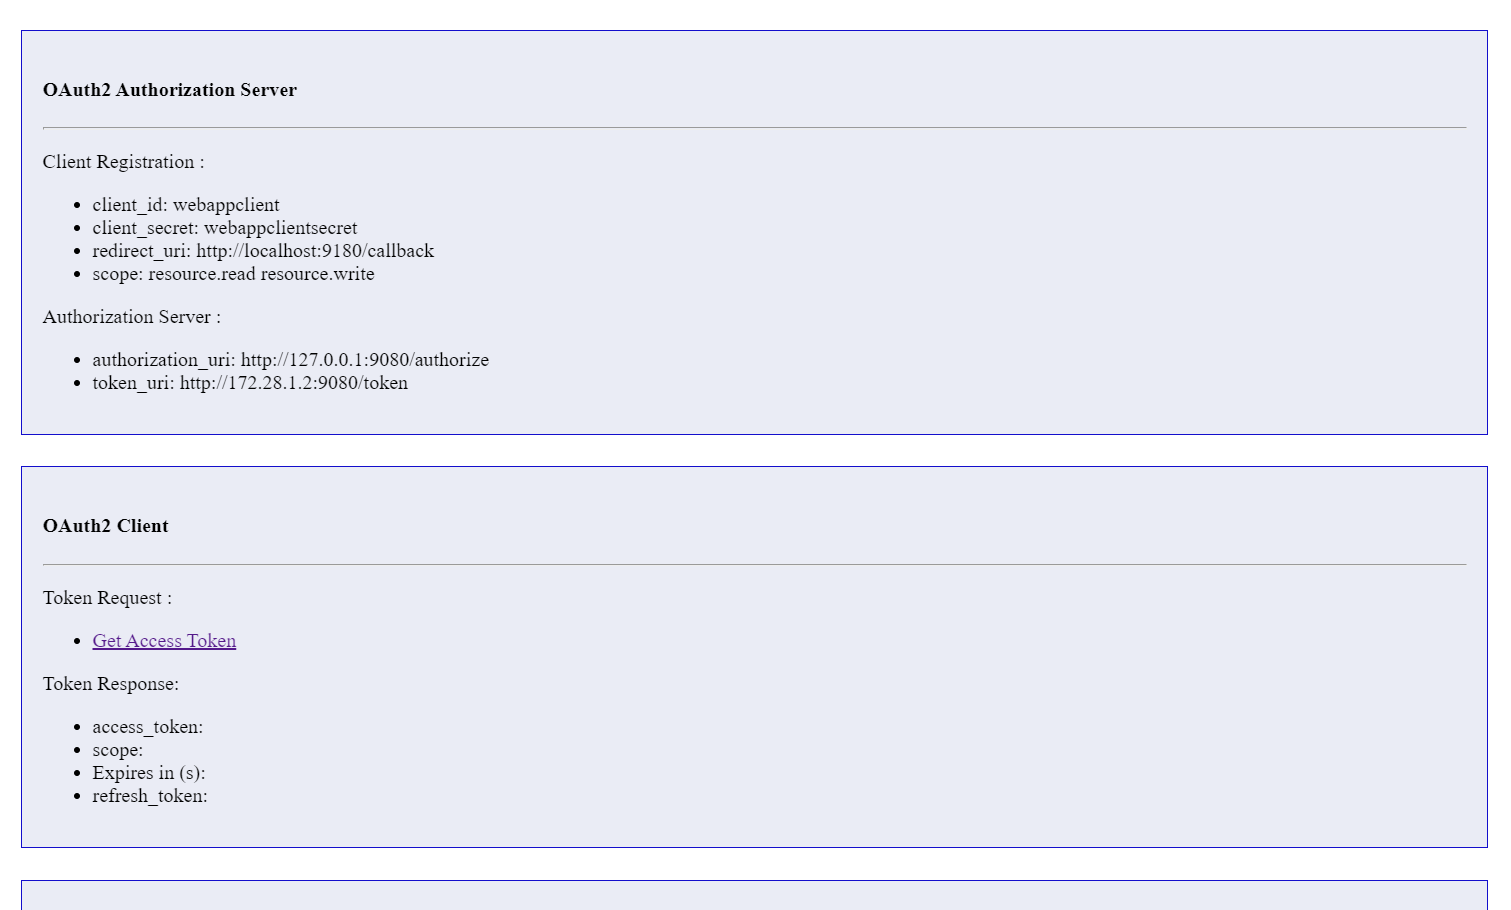
\includegraphics[scale=0.50]{chapters/images/chp5/screen2.png}}
    \caption{The homepage of the second implementation example}
    \label{fig:home2}
\end{figure}

\noindent Since this is an educational example, all the information are in plain text in the homepage. The first thing to do is to retrieve the access token by clicking on the link. Then, a log-in is necessary. The only available credentials are:

\begin{itemize}
    \item Username: \textit{appuser}
    \item Password: \textit{appusersecret}
\end{itemize}

\noindent After the log-in, it is displayed a checkbox in order to select what authorizations will be delegated to the client app. Select \texttt{resorce.read}, \texttt{resource.write} or both. 
Finally, the user will be redirected to the homepage with an access token. Now, it is time to request the resource using the two links at the end of the page. If the client is authorized, it will print a simple message, otherwise a 403 HTTP error is displayed (Forbidden). In addiction, it is available the refresh token flow based on the authorized resources or a subset of them (e.g. if someone has the access token for both scopes, it can make the token refresh for only one too). To stop the application and safely detach all the resources, \texttt{Crtl+C} command on the terminal and finally:

  \texttt{\$ docker-compose down}

\noindent The full screen video captioning of the example is available in the Assets of the releases page\footnote{\scriptsize{\url{https://github.com/nopesir/oauth-hw-security-custom/releases/download/v0.5-alpha/hw-security-custom-screen.mp4}}} or in the resources. 
% ------ END OF SECTION A.2.2 ------
% ------ END OF SECTION A.2 ------

% ------ END OF APPENDIX A ------
    
    % ------ APPENDIX B ------

\chapter{Programmer manual}
% ------ APPENDIX INTRO ------
This appendix explains how the two implementations are designed. In particular, there is a first section about the frameworks and the libraries used, followed by the implementation itself (with code explanations, problems, resolutions, endpoints and messages exchanged in practice) for both the examples. Finally, the last section is devoted to the compilation and dockerization of the solutions.
% ------ END OF APPENDIX INTRO ------

\minitoc

% ------ SECTION B.1 ------
\section{Frameworks, libraries and environment}
For what concerns the second demo and the server of the first demo, it has been used Apache Maven as build automation tool and the only requirement is Java JDK8 installed. Moreover, since Maven is integrated into the project (by using maven-wrapper), there is no need to install it on the machine.
For what concerns the client in the first demo, React is the Javascript framework chosen. The programs \texttt{npm} and \texttt{node} must be installed on the machine (see \url{https://www.npmjs.com/get-npm} to get both of them). 
The code of the implementation examples is available on GitHub:

\begin{itemize}
    \item \textbf{\oauth\ with Google/Facebook}\footnote{\url{https://github.com/nopesir/oauth-hw-security}}
    \item \textbf{\oauth\ with custom AuthZ/Resource servers}\footnote{\url{https://github.com/nopesir/oauth-hw-security-custom}}
\end{itemize}

Last but not least, both \texttt{Docker} and \texttt{Docker-Compose} must be installed too to dockerize the solutions. For instructions, see (\ref{appa}).
% ------ END OF SECTION B.1 ------

% ------ SECTION B.2 ------
\section{Implementation}
In this section are analyzed the design and implementation of the two solutions with messages exchanged and endpoints used. The "Playground" demo provided by OAuth.com in collaboration with Okta \cite{playgr} can be very helpful for the developer to understand the flows and the protocol from a practical point of view. 

% ------ SECTION B.2.1 ------
\subsection{\oauth\ with Google/Facebook}
The \textit{server-side} is a Spring Boot application that uses \oauth\ by exploiting Spring Security in order to implement both social (Google/Facebook/GitHub) and email/password logins (with a MySQL database). On the other hand, the \textit{client-side} application is not strictly related to \oauth, but it is an example on how to use the information provided by the \oauth\ Spring Boot server to interact with an end-user (in this case, a React web application). Since the flow with some providers varies for what concerns payloads types and endpoints, of particular relevance are the official documentations from Facebook \cite{facebook} and Google \cite{google1, google2}. Furthermore, to implement the Spring Boot server, a good example can be found on the developer.okta.com's blog \cite{sprboot}. 

\subsubsection{Client-side}

\begin{wrapfigure}[20]{r}{0.31\textwidth}
  \begin{center}
    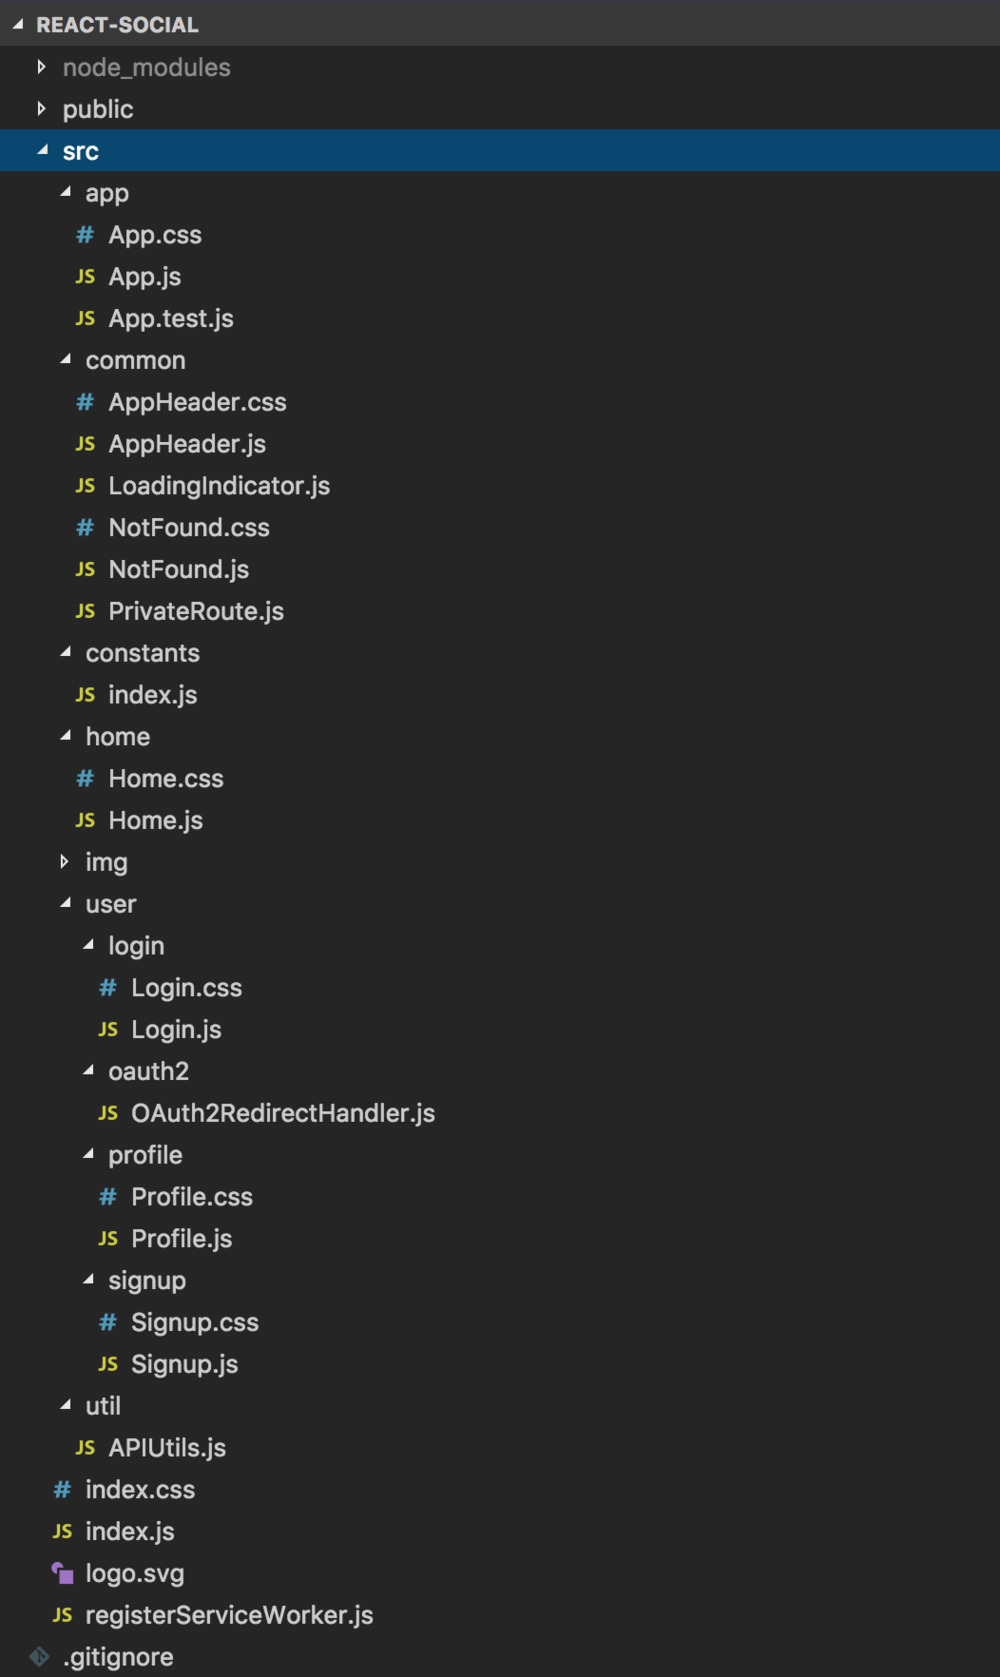
\includegraphics[width=0.31 \textwidth]{chapters/images/chp6/dirreact.jpg}
  \end{center}
  \caption{Final directory tree of the \texttt{react-social} app}
  \label{fig:dirtree}
\end{wrapfigure}

As mentioned before, this application is pretty simple and it is only used as an interface between the \oauth\ Spring Boot back-end server and the user to display information. An alternative could be directly to implement into the Spring Boot back-end the web-server.

\noindent To create the base React application, simply type:
\begin{lstlisting}[language=bash]
  $ npm install -g create-react-app
  $ create-react-app react-social
\end{lstlisting}

\noindent And then add the dependencies for routing and alerts:
\begin{lstlisting}[language=bash]
  $ cd react-social
  $ npm install react-router-dom react-s-alert --save
\end{lstlisting}

\noindent That is the base React application to build on. We have to populate and organize the final directory structure to look like in Fig.~\ref{fig:dirtree}.

The code is pretty self-explanatory, but there are some important aspects to consider. The first one is \textbf{index.js}, that is the entry-point of the application. It renders the App component in a document object model that has \texttt{root} as id and it is subsequently wrapped into a Router to enable client-side routing. The second important aspect is \textbf{App.js}, located in \texttt{src/app}. It is the top-level element of the application and is responsible for the layout, the routes and manages the authentication by loading the details from the back-end of the current user, forwarding it to the child components. The \textbf{Login.js} file, located in \texttt{src/user/login}, is responsible for the \oauth\ login and the username/password login, while \textbf{OAuth2RedirectHandler.js} is the component called by the Spring Boot server when the user has completed the \oauth\ flow on it. In particular, once that the server flow is finished, the server saves all the information in a database and generates a local token. This component will receive a bearer token from the Spring Boot server (note that this token is not related to \oauth, it is a token generated by the Spring Boot server to manage the access to the database information) or an error otherwise.

Last but not least, the \textbf{index.js} located in \texttt{src/constants} contains information about the endpoints. The \texttt{API\_BASE\_URL} refers to the Spring Boot server base URL, that represents the API for the \texttt{hw-client} app. The \texttt{OAUTH2\_REDIRECT\_URI} is the redirection URI where the \\ \textbf{OAuth2RedirectHandler.js} is waiting to handle the response and the three \texttt{PROVIDER\_AUTH\_URL} are the Spring Boot server URLs called when the user clicks on one of the three \oauth\ login, passing as parameter a \texttt{redirect\_uri} to let the server know where to redirect the local token once that he has completed the AuthZ Code Grant flow. 

\begin{figure}[h!]
    \centering
    \fbox{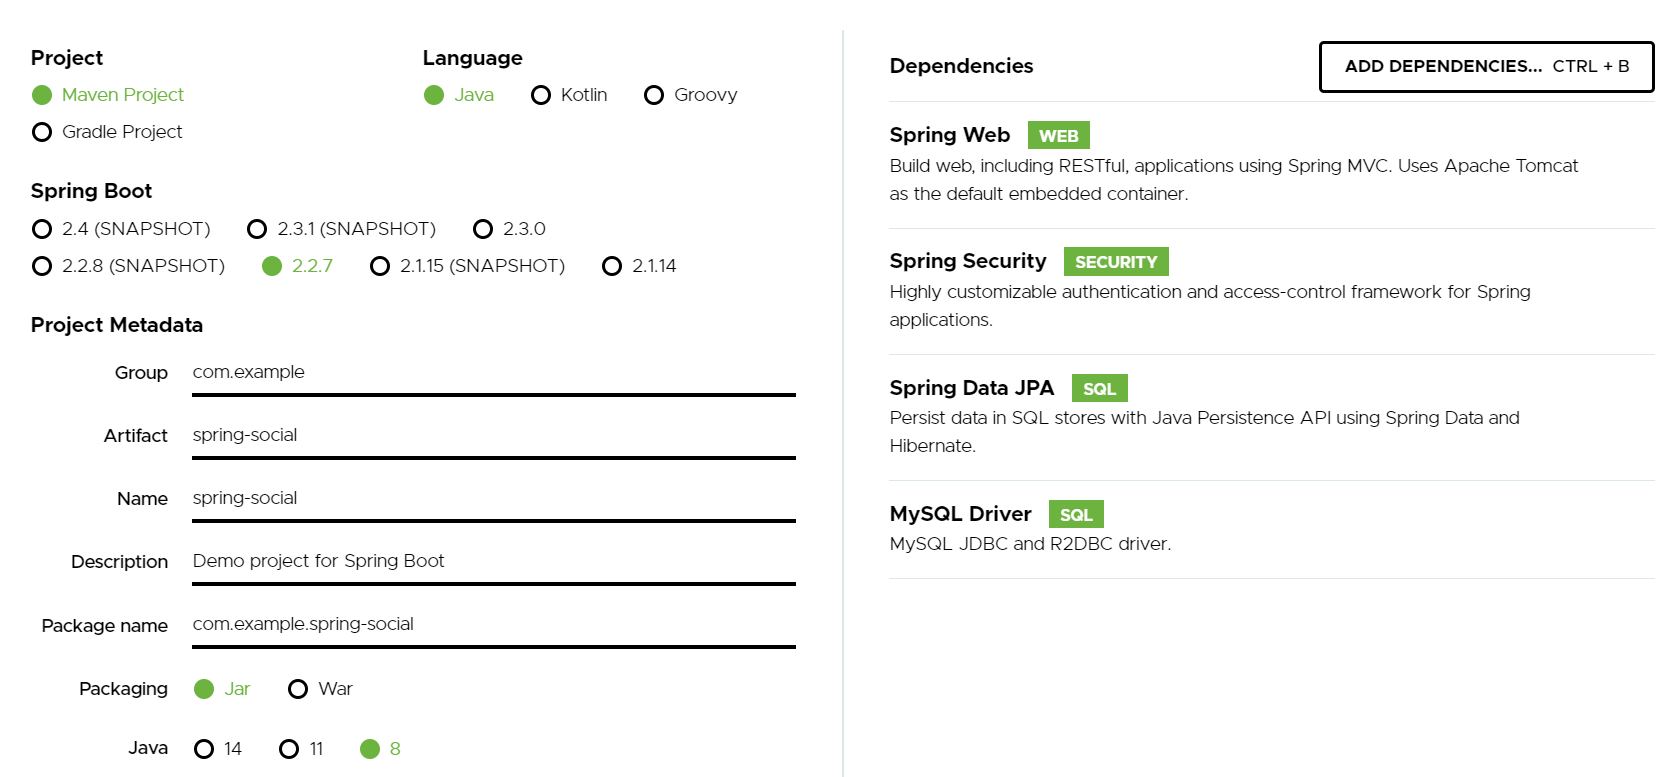
\includegraphics[width=16cm]{chapters/images/chp6/spring.png}}
    \caption{Spring Boot base project selection}
    \label{fig:spring}
\end{figure}

\subsubsection{Registration process}
To enable the Spring Boot server to perform a social login with an \oauth\ provider, the first step is to create an application in the provider's developer console and obtain the \texttt{client\_id} and \texttt{client\_secret}. These two strings are used by the providers (Google, Facebook and so on) to identify our server application. Besides, there are some other parameters to consider:

\begin{itemize}
    \item Authorized redirect URIs: After that the AuthZ Grant Flow finishes, the provider needs this URI to understand where the user has to be redirected after the flow and what are the ones that are authorized by the developer.
    \item Scopes: They represent \textbf{what} can be granted. Note that this is only meant to enable the possibility to give it, it is not automatically given to our server. The user will decide what scopes from the enabled scopes can be consumed by the Spring Boot server.
\end{itemize}

\noindent To create an app, simply start a new app in one of the following provider's page:

\begin{itemize}
    \item Google Project: \url{https://console.developers.google.com/}
    \item Facebook: \url{https://developers.facebook.com/apps}
    \item GitHub: \url{https://github.com/settings/apps}
\end{itemize}

\noindent Set the Authorized redirect URIs (more on this in the next subsection), the scopes (email, name) and retrieve the two secrets for each provider.

\subsubsection{Server-side}

\begin{wrapfigure}[15]{r}{0.3\textwidth}
  \begin{center}
    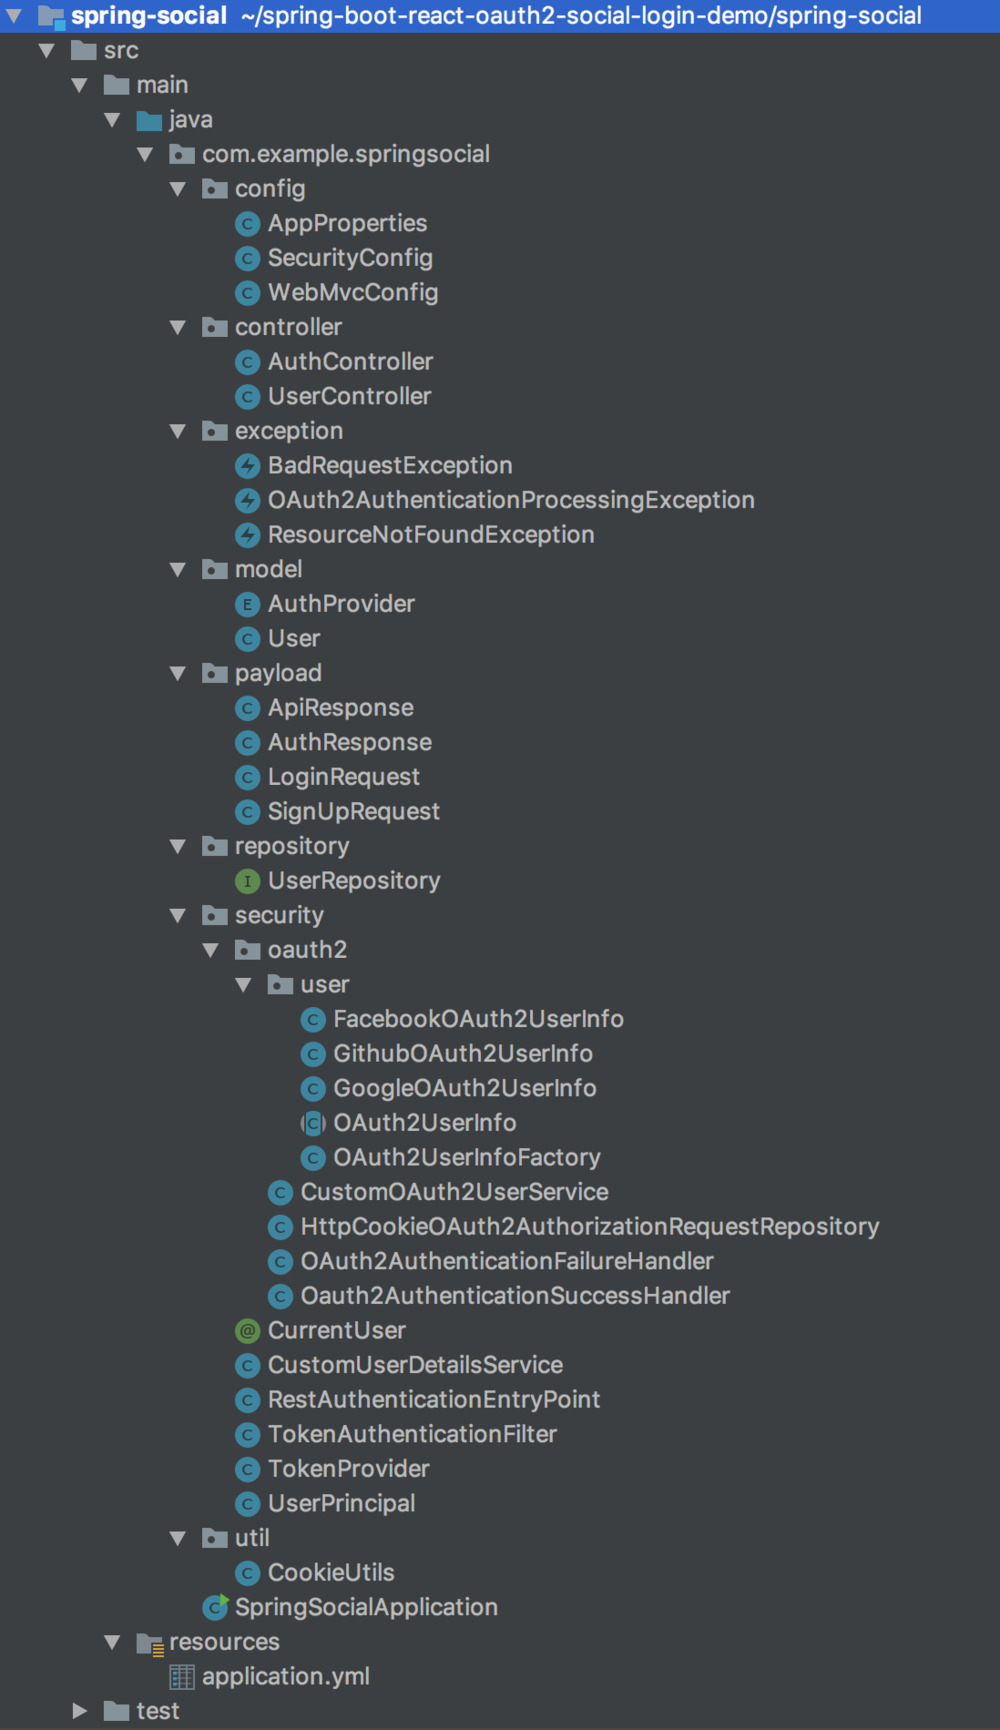
\includegraphics[width=0.3 \textwidth]{chapters/images/chp6/springdir.jpg}
  \end{center}
  \caption{Final directory tree of the \texttt{spring-social} app}
  \label{fig:dirsocial}
\end{wrapfigure}

The server, as it has already mentioned, is a Spring Boot application. The base project can be automatically created using Spring Initializr\footnote{Start the project from \url{https://start.spring.io/}}. In particular, the selections are the ones in Fig.~\ref{fig:spring}.

Then, the project folder has been modified to have the directory structure in Fig.~\ref{fig:dirsocial}. Furthermore, two more dependencies must be added to the project (not available on Spring Initializr): \textit{\oauth\ Client} and \textit{JWT Library}. By opening the \texttt{pom.xml} file, thanks to Maven, simply add these lines into the \texttt{<dependencies></dependencies>} tags:

\begin{lstlisting}[language=XML, basicstyle=\fontsize{9}{11}\ttfamily]
  <!-- OAuth2 Client -->
  <dependency>
    <groupId>org.springframework.security</groupId>
    <artifactId>spring-security-oauth2-client</artifactId>
  </dependency>

  <!-- JWT library -->
  <dependency>
    <groupId>io.jsonwebtoken</groupId>
    <artifactId>jjwt</artifactId>
    <version>0.5.1</version>
  </dependency>
\end{lstlisting}

\noindent Now that the Spring Boot app structure is ready, we are going to analyze every Java file and configuration file to understand how the functionalities are implemented. The configuration file is \textbf{application.yml} (note that if a file has \texttt{.template} as extension it represents a simple file without this extension with some variables to be changed at build time, see \ref{docker} for more information). The configuration file is located in \texttt{src/main/resource/} and it contains all the information about the database, the redirection URIs and so on. In \texttt{spring.datasource} are saved the MySQL database variables, while in \texttt{spring.security.oauth2} we can find everything that concerns \oauth\ providers and their details. In particular, for each provider, we can insert the two secrets (\textit{clientId} and \textit{clientSecret}) with the redirect URI and the scopes.

In a few words, all the content stored in \texttt{spring:} is related to the server itself, while \texttt{app:} is used to authenticate the React web application. More in details, \texttt{app.auth} information is consumed for the creation of a JWT authentication token (that has nothing to do with \oauth) that is passed to the React front-end (or any other front-end, as a mobile app) by a redirection to \\ \texttt{http://localhost:9090/oauth2/redirect} (enabling OAuth2RedirectHandler.js) or for example \texttt{myandroidapp://oauth2/redirect} if the front-end is a mobile app.
After successfully authenticating with the \oauth\ Provider, the Spring Boot server will generate an auth token for the user and will send the token to the \texttt{redirectUri} mentioned by the front-end client in the \texttt{/oauth2/authorize} request. 

The next step is to load this configuration file and bind the properties. The \\ \texttt{@ConfigurationProperties} feature is used in \textbf{AppProperties.java} to load the \texttt{app:} information from the configuration file and is enabled with  \texttt{@EnableConfigurationProperties} in the main file \textbf{SpringSocialApplication.java}. Moreover, to enable CORS\footnote{Cross-Origin Resource Sharing, "[...] a mechanism that uses additional HTTP headers to tell browsers to give a web application running at one origin, access to selected resources from a different origin.". Source: \url{https://developer.mozilla.org/en-US/docs/Web/HTTP/CORS}} is created a \textbf{WebMvcConfig.java}  so that our front-end can access the APIs from different origins. The used restrictions are pretty low for the demo, but in production environments they must be restricted.

To enable the database interaction, the database entities must be created. The User entity is available in the \textbf{User.java} file, alongside the \texttt{enum} \textbf{AuthProvider.java} that represents the provider. The implementation of the database functionalities is denoted to the \textbf{UserRepository.java} interface. Here it is used \textit{Spring-Data-JPA} to build a repository layer to access the database information.
Once that the configuration, the entity classes and repositories are ready, we will use Spring Security to perform the \oauth\ social login as well as the password/email based login.

The core of the \oauth\ Security on the server is \textbf{SecurityConfig.java}, that binds all the constituents to implement a security policy for the entire application. In particular, the \textit{SecurityConfig} is an extension to a  \textit{WebSecurityConfigurerAdapter} and overrides some of its methods to provide custom security configurations:

\begin{itemize}
    \item \textit{CustomUserDetailsService}
    \item \textit{CustomOAuth2UserService}
    \item \textit{OAuth2AuthenticationSuccessHandler}
    \item \textit{OAuth2AuthenticationFailureHandler}
    \item \textit{HttpCookieOAuth2AuthorizationRequestRepository}
    \item \textit{TokenAuthenticationFilter}
    \item And all the classes implemented in \texttt{java.com.example.springsocial.security}
\end{itemize}

\noindent The flow starts with the front-end client. After that one of the three available \oauth\ login buttons is clicked, the React app redirects the user to \\

\vspace{0.1cm}

\hypertarget{foo}{}

\texttt{\footnotesize{http://localhost:8080/oauth2/authorize/\{provider\}?redirect\_uri=<redirect\_uri\_after\_login>}} \\

\vspace{0.1cm}

\noindent Where \texttt{localhost:8080} is the Spring Boot server base URL, \texttt{provider} represents one of the three providers and the \texttt{redirect\_uri} is the URI to which the user will be redirected after the \oauth\ flow on the provider site (note that this redirection is not the \oauth\ \texttt{redirectionUri}).

Once that the authorization request is received, Spring Security's \oauth\ redirects the user on the \textit{AuthorizationUrl} of the \texttt{provider} with some parameters (the scopes and the redirectionUri saved in the configuration file). Here, \textit{authorizationRequestRepository} applies persistency to the request's state. The user is now on the provider's login/authorization page, where it can log in and allow/deny permission to the Spring Boot server. Once that it allows it, the provider sends the user to \texttt{\{baseUrl\}/oauth2/callback/provider} with an AuthZ code (or an error otherwise).

At this point, \textit{oAuth2AuthenticationFailureHandler} is invoked in case of failure (it redirects the user on the React app with an err message in the query string), otherwise, the flow continues and the previous callback contains the \texttt{authorization\_code} that is automatically exchanged by Spring Security for an \texttt{access\_token}. The next step is \textit{customOAuth2UserService} that takes all the details of the authenticated user by performing HTTP GETs to the defined endpoints available in the Google/Facebook documentation and adds/updates the database. Spring Security is really useful in this objective because it has already implemented the HTTP API calls for the most famous providers and it is almost automated. 

Finally, the last step is \textit{oAuth2AuthenticationSuccessHandler}, that creates a JWT token and sends it to the React app's \texttt{redirect\_uri} previously sent at the beginning. Once that the client app receives it, it can make an HTTP GET with the JWT on the endpoint of the Spring Boot server \texttt{/user/me} to retrieve the user information and display it to the client. The generic flow with Google is available in \texttt{.svg} format\footnote{\url{https://github.com/nopesir/oauth-hw-security/releases/download/v0.5-alpha/flow.svg}}.


In Section \ref{csrf} has been discussed the problem of CSRF. In particular, the recommended way of avoiding this kind of attack is the use of a \texttt{state} parameter. When the Spring Boot server redirects the user to the provider's login page (see \hyperlink{foo}{here} the HTTP redirection link), it has to first generate this string variable and send it as HTTP parameter with the \texttt{redirect\_uri}. The provider must return this parameter unaltered in the \oauth\ callback and the server will compare the generated one with the received one. In case they don't match, the flow is stopped and the request denied.
The class \textit{HttpCookieOAuth2AuthorizationRequestRepository} temporary stores the \texttt{redirection\_uri} and the \texttt{state} params in a short-lived cookie.

To gain access to the user's info, the \textit{CustomOAuth2UserService} implements the Spring Security's \textit{DefaultOAuth2UserService} by its \texttt{loadUser()} method (called after that an \oauth\ \texttt{access\_ token} is finally available). More in details, the method fetches what is needed from the provider and then checks the database to update it. Since the JSON structure of the responses of each provider changes, Spring Security provides a parsing layer that returns a map of key-value pairs. To manage the different providers, a generic \textit{OAuth2UserInfo} is created and a factory design pattern is implemented through \textit{OAuth2UserInfoFactory} to instantiate the correct \textit{OAuth2UserInfo} (\textit{GoogleOAuth2UserInfo}, \textit{FacebookOAuth2UserInfo}, \textit{GithubOAuth2UserInfo}).

In addition to the \oauth\ login, the Spring Boot server implements the classic email/password based authentication. The class \textit{AuthController} is responsible for controlling the REST endpoints \texttt{/auth} and \texttt{/signup}, while the \textit{CustomUserDetailsService} implements \textit{UserDetailsService} to load the user from the database. For managing (generate/verify) the JWT tokens, a \textit{TokenProvider} is created. Moreover, the \textit{TokenAuthenticationFilter} class uses the provider one to verify the JWT and set the \texttt{SecurityContex}. \textit{RestAuthenticationEntryPoint} checks for unauthorized accesses and returns a 401 HTTP error for it. The \textit{UserPrincipal} class contains the details of the authenticated user while \textit{UserController} implements the API for retrieving the details of it. Finally, there is a utility class that is used for the cookies management called \textit{CookieUtils}. \textit{LoginRequest}, \textit{SignUpRequest}, \textit{AuthResponse} and \textit{ApiResponse} are the request/response payloads.

For further information on Spring Security, see the documentation \cite{sprsec}.
% ------ END OF SECTION B.2.1 ------

% ------ SECTION B.2.2 ------
\subsection{\oauth\ with custom AuthZ/Resource servers}
This second implementation example is required to better understand \oauth\ and his actors without the customization of providers like Google. It is possible to build an authorization server and a resource server using the \textit{authorization grant flow} (\ref{authcg}). For this task, before using directly the \rfc{6749}, the developer.okta.com's article "What is the OAuth 2.0 Authorization Code Grant Type?" \cite{oauth2} is a good start. The demo is composed by three servers:

\begin{itemize}
    \item \textit{Client-server}, that acts like the Spring Boot server in the previous example (the client of the \oauth\ protocol specification that is interested in accessing a resource), but without a React web app: it is used a classic routing website served directly from the server itself.
    \item \textit{Authorization-server}, that provides endpoints for user authentication and authorization, token access and token refresh and so on.
    \item \textit{Resource-server}, that makes available resources by using the retrieved token from the authorization server.
\end{itemize}

There is the user too (the resource owner), that is responsible for grant/deny permissions to the client-server. All the software of this demo uses Maven for project management, dependencies and so on. Moreover, it is built on top of \texttt{Jakarta EE} \cite{jaksec} with \texttt{MicroProfile}, but more details are available in the dedicated subsections. 

\subsubsection{Client-server}
This web-server implements four Servlets\footnote{Exploit dynamic web content with Java, "[..] class that is used to extend the capabilities of servers that host applications accessed employing a request-response programming model.". Source: \url{https://docs.oracle.com/javaee/5/tutorial/doc/bnafe.html}}:

\begin{itemize}
    \item Request the authorization code from the authorization server's endpoint.
    \item Request the access token by consuming the authorization code.
    \item Request the access token by consuming the refresh token (\ref{accref}).
    \item Request the resource from the resource server's endpoint by consuming the access token.
\end{itemize}

\noindent Moreover, it uses MicroProfile Config for configuration files injection and JAX RS Client for accessing web resources. For simplicity, the \texttt{client\_id} and \texttt{client\_secret} are manually defined in the authorization server as it will be explained in the next subsection. This means that our client must have securely stored the two secrets that, for this demo, are only one pair (since the client is only one). In the configuration file stored in \texttt{META-INF/microprofile-config.properties} (it must be noted that it applies the same \texttt{.template} design, as explained in the first demo), apart from the secrets, other important variables are:

\begin{itemize}
    \item \texttt{redirect\_uri}: As it was already mentioned, this is \textit{where} to receive the AuthZ code.
    \item \texttt{scope}: The permission requested by the client.
    \item \texttt{authorization\_uri}: The client needs to know where to send the request for the AuthZ code.
    \item \texttt{token\_uri}: As for the AuthZ URI, the client needs to know where to send the request to exchange the code for an access token.
\end{itemize}

\noindent It is important though to point out that the URIs are configured for the Docker virtualized network and they need to be changed to be run without Docker.

The first Servlet implements the AuthZ code request on the AuthZ server's endpoint and it is represented by the \textit{AuthorizationCodeServlet} waiting to start on the \texttt{/authorization} endpoint of the client. More in details, the Servlet creates and stores the \texttt{state} param, retrieves the information from the MicroProfile Config file and builds the URI attaching all the variables. Finally, it redirects the user to the built URI (that is on the AuthZ server). After processing the request, the AuthZ server will redirect back the user to the client with the AuthZ code and the same \texttt{state} param on the URI \texttt{http://localhost:9180/callback?code=tughdj57gh5hfd\&state=57t7fdhgwejgu54h} where the second Servlet is waiting for the AuthZ code (the client server is on 9180, the AuthZ server is on 9080 and the resource server on 9280).

The second Servlet starts as soon as the AuthZ server redirects back to \texttt{/callback} with the AuthZ code and the \texttt{state} as parameters. The implementation is in class \textit{CallbackServlet}. First, it checks the \texttt{state} match and then it uses the received code to request an access token. In this case, there is no browser interaction, it is all implemented through HTTP POST and JAX RS Client: here the token endpoint requires the two secrets too in the \textit{Authentication} header, along with the code, the type of the code and the redirect URI. Now the client has the access token (and the refresh token too) and it can access information on the resource server by using the third Servlet implemented in \textit{DownstreamCallServlet} waiting on \texttt{/downstram} with two actions passed as query params: \textit{read} or \textit{write}. Based on the action, the Servlet calls the resource server's APIs with the access token in the Authorization HTTP header and receives a string if it has access or an HTTP Forbidden error if it does not.

The last Servlet is used to obtain a new access token starting from the refresh token. This is useful because it does not require the user to repeat all the flow. The Servlet is ready to start at \texttt{/refreshtoken} and, similarly to the code of \textit{CallbackServlet}, it uses only JAX RS Client and HTTP POST to build the request, that has the refresh token, the scopes and as grant type \texttt{refresh\_token}. The Authentication header with the encoded secrets is added too. The request is posted on the same token endpoint of the AuthZ server, but the AuthZ server will know what to do because of the \texttt{grant\_type} param. If the response is 200 HTTP, the new token is stored and it can be used for the next calls to the resource server.

To start the first Servlet and/or to know every parameter and token for educational purposes, a simple homepage is built (\texttt{src/main/webapp/index.jsp}) that in a few words prints all the information and makes available the endpoints (by mouse click) to the user.

\subsubsection{Authorization-server}
This server is the core of the \oauth\ implementation. For simplicity, a pre-configured client and a pre-configured user are used, stored in \texttt{src/main/resources/data.sql.template} (it must be pointed out though that for a production environment the passwords must be hashed). 

The first important endpoint is the AuthZ endpoint that is responsible for the authentication of the user to subsequently ask for the needed permissions. The Section 3.1 of the \rfc{6749} states that "The authorization server MUST support the use of the HTTP "GET" method [\rfc{2616}] for the authorization endpoint and MAY support the use of the "POST" method as well.". In this implementation is preferred the HTTP GET method alone. Since the specification does not ask for a particular login flow, a simple login form with Jakarta EE Security can be used. The class \textit{AuthorizationEndpoint} contains:

\begin{itemize}
    \item \texttt{@FormAuthenticationMechanismDefinition} to ensure that the user is logged to proceed.
    \item HTTP GET Servlet that checks the validity of the secrets, the redirect URI, the requested scope and saves all this params in the session and redirects the user to the \texttt{authorization.jsp} from where it selects what to authorize with some checkboxes.
    \item HTTP POST Servlet that receives the user checkboxes from \texttt{authorization.jsp}, uses the saved params in the preceding point to populate a new AuthZ code model with the authorization code, the \texttt{client\_id}, the approved scopes, the expiration date and so on and redirects back to the client on the \texttt{redirect\_uri} by adding to the query params the new code alongside the state received at the beginning for avoiding CSRF. The \texttt{redirect\_uri} must exist in the table as an authorized URI for redirections.
\end{itemize}

\noindent As mentioned before, retrieving the access token starting from the authorization token is an action that does not require the user nor the browser intervention. The token endpoint of the AuthZ server, under the client-server, uses JAX RS to expose the endpoint. The class \textit{TokenEndpoint} implements the next step of the workflow: retrieve the access token. The Servlet accepts only HTTP POST and, as mentioned in the \oauth\ specification, accepted parameters mus be \texttt{application/x-www-form-urlencoded}. The first thing that the Servlet checks are the \texttt{grant\_type} that must be \texttt{authorization\_code} since this is an AUthZ Code Grant flow implementation. The second check is on \texttt{client\_id} and \texttt{client\_secret} that are in the Authorization header of the received post (this is required by the protocol to identify the client). The two secrets are encoded into Base64url following this conversion:
\begin{lstlisting}
  BASE64URL(client_id:client_secret)
\end{lstlisting}

\noindent Finally, the Servlet creates the access token by using \textit{AuthorizationCodeGrantTypeHandler}. 

Since the endpoint can and should be used for both the requests of getting an access token starting from an authorization code or getting an access token starting from a refresh token, the Servlet must be dynamically capable of choosing the right class instance. A possible solution is an implementation through the Contexts and Dependency Injection (CDI). More in details, an \textit{AuthorizationGrantTypeHandler} interface is created and implemented with \textit{AuthorizationCodeGrantTypeHandler} for AuthZ code to access token and with \textit{RefreshTokenGrantTypeHandler} for refresh token to access token. Each class is decorated with the \texttt{@Named} that specifies for the first one the \texttt{authorization\_code} type and the second one the \texttt{refresh\_token} type. By using the decoration, in the Servlet can be written a single line of code that uses the received string (\texttt{grantType}) on the endpoint and uses it directly to load one handler or the other one:

\noindent \texttt{\footnotesize{AuthorizationGrantTypeHandler authorizationGrantTypeHandler= \\
\indent authorizationGrantTypeHandlers.select(NamedLiteral.of(grantType)).get();}} 

\noindent To generate tokens though, it is required that the server signs them with a private RSA key. It has been used OpenSSL to generate the private key:

\begin{lstlisting}[language=bash, basicstyle=\fontsize{9}{11}\ttfamily]  
  $ openssl genpkey -algorithm RSA -out private-key.pem -pkeyopt rsa_keygen_bits:2048
\end{lstlisting}

\noindent And the path to this key is saved in \texttt{resources/META-INF/microprofile-config.properties} to be injected into the server configuration info to be loaded directly from the code. Alongside the private key, a corresponding public key is generated:

\begin{lstlisting}[language=bash, basicstyle=\fontsize{9}{11}\ttfamily]  
  $ openssl rsa -pubout -in private-key.pem -out public-key.pem
\end{lstlisting}

\noindent And stored in the same configuration file.

When the resource server receives a request with an access token for a resource, it has to verify it by using the public key. Another endpoint is necessary on the AuthZ server: a JWK [\rfc{7517}] for public key distribution. This endpoint is mapped in \texttt{/jwk} and the Servlet is implemented by the class \textit{JWKEndpoint}. Thanks to the Nimbus library, the code is much more simplified with both the JWT and PEM formats compatibility (by specifying the param \texttt{format} in the URI query).

For what concerns the authorization endpoint, it was already mentioned the existence of the \texttt{AuthorizationGrantTypeHandler}, but how does it work? What does the endpoint returns? More in details, it uses the Nimbus JOSE library for creating a JWT token. The first thing to do is to create a JWT header and then populate the payload with some claims (like the issuer, the claimer and so on). Then, the token must be signed with the RSA Private Key. This step can be divided into two: 

\begin{itemize}
    \item The JWT is created starting from the claims and the header.
    \item The \textit{RSASSASigner} object uses the imported PEM key to sign the JWT.
\end{itemize}

\noindent Finally, the JWT is ready and it is serialized into a \textit{String}. More in details, this serialization follows the "JWS Compact Serialization" defined in Section 7.1 of the \rfc{7515} \cite{RFC7515}:

\begin{lstlisting}
  BASE64URL(UTF8(JWS Protected Header)) || '.' ||
  BASE64URL(JWS Payload) || '.' ||
  BASE64URL(JWS Signature)
\end{lstlisting}

\noindent An example of a valid serialized JWT for this implementation could be:

\begin{lstlisting}
  eyJ0eXAiOiJKV1QiLCJhbGciOiJSUzI1NiJ9
  .
  eyJzdWIiOiJhcHB1c2VyIiwiYXVkIjoiaHR0cDpcL1wvMTcyLjI4LjEuMzo5Mjg
  wIiwidXBuIjoiYXBwdXNlciIsIm5iZiI6MTU5Mzc5MDY1MSwic2NvcGUiOiJyZX
  NvdXJjZS5yZWFkIiwiaXNzIjoiaHR0cDpcL1wvMTcyLjI4LjEuMjo5MDgwIiwiZ
  3JvdXBzIjpbInJlc291cmNlLnJlYWQiXSwiZXhwIjoxNTkzNzkyNDUxLCJpYXQi
  OjE1OTM3OTA2NTEsImNsaWVudF9pZCI6IndlYmFwcGNsaWVudCIsImp0aSI6ImI
  3MmNiOTc2LTgxY2ItNGRjNi1hMjMwLTg2YzE2ZTE1NWQyNiJ9
  .
  pVjwobEPgfjLMdVHdBKNhwNcqpG9UytZH2wcJYtVuVFitgaDk6cWwTCCJlOLLO
  qcvtXsl4RjXavKFFGVIalQL1Smqj69u6i98VqRVn6yRiPyi8EDJeJn6Xa2BjIF
  ePjPc8EyejvM47F0LDwJO19kb-s8fcXKqEdB0zTQ8vMvb-1jgk9KlXWzsT3HxN
  rRLnpHyUAWjELVe30awwF0v9MfGPdxX64Kq62hNA2hg8TLLHXWEgU1v5eqCmdk
  sD1kyhS_cPSQLRKcXQMDPdTe1H4cnXnm8Gl_qYV885RYLx0DXqddWoiRPCLu
  5RbLr2ZXxAOSFQ8kKScmXX3BUpkiHS5afw

  
\end{lstlisting}

\noindent Where the first part of the string is the Base64url encoded JOSE Header that specifies the used algorithm and the type. The decoded string would be:

\begin{lstlisting}
  {
    "typ":"JWT",
    "alg":"RS256"
  }
\end{lstlisting}

\noindent The second part represents the encoded JWS Payload with all the previously built claims, decoded as:

\begin{lstlisting}
  {
    "sub":"appuser",
    "aud":"http://172.28.1.3:9280",
    "upn":"appuser",
    "nbf":1593790651,
    "scope":"resource.read",
    "iss":"http://172.28.1.2:9080",
    "groups":["resource.read"],
    "exp":1593792451,
    "iat":1593790651,
    "client_id":"webappclient",
    "jti":"b72cb976-81cb-4dc6-a230-86c16e155d26"
  }
\end{lstlisting}

\noindent Where, according to the \rfc{7519}\ specification \cite{RFC7519}, are defined the following Registered Claim Names:

\begin{itemize}
    \item \texttt{sub}: OPTIONAL. The principal that is the subject to the JWT.
    \item \texttt{aud}: OPTIONAL. Audience, to whom the JWT is addressed.
    \item \texttt{nbf}: OPTIONAL. Not Before, "the time before which the JWT MUST NOT be accepted for processing." \cite{RFC7519}
    \item \texttt{iss}: OPTIONAL. The issuer of the JWT.
    \item \texttt{exp}: OPTIONAL. The expiration time.
    \item \texttt{iat}: OPTIONAL. Issued At.
    \item \texttt{jti}: OPTIONAL. JWT ID, a unique identifier for the JWT.
\end{itemize}

\noindent And the following Private Claim Names designed for the demo:

\begin{itemize}
    \item \texttt{upn}: To be mapped into Jakarta EE Security \textit{CallerPrincipal}.
    \item \texttt{groups}: To be mapped into Jakarta EE \textit{Roles}.
    \item \texttt{client\_id}: The ID of the \oauth\ web-server client.
\end{itemize}

\noindent These claims are built in the token endpoint response code in the \textit{AbstractGrantTypeHandler} class. For what concerns the \texttt{refresh\_token}, the JWT is similar, with few claims and expiration of one day.
Finally, the third and last part of the JWT represents the Base64url encoded JWS Signature performed by the server on the following octets:
\begin{lstlisting}
  ASCII(
    BASE64URL(UTF8(JWS Protected Header)) || '.' ||
    BASE64URL(JWS Payload)
  )
\end{lstlisting}

\noindent Those octets are signed using RSASSA-PKCS1-v1\_5 with the SHA-256 hash algorithm (defined as \texttt{RS256} in the JOSE Header) by the server and finally encoded in Base64url.

The last thing to do is build the JSON response and add the elements and the serialized JWTs (refresh and access tokens) to return the information requested by the client. This step is implemented into the \textit{AuthorizationCodeGrantTypeHandler} class, that once it has serialized the two JWTs, it builds the response:

\begin{lstlisting}[language=bash, basicstyle=\fontsize{12}{14}\ttfamily]
  {
    "access_token": "averylongstring,seepage46" ,
    "token_type": "Bearer",  
    "expires_in": 1800,
    "scope": "resource.read",
    "refresh_token": "smallerthanaccesstoken,lessclaims"
  }
\end{lstlisting}

A detailed diagram of the AuthZ Code Grant flow for this implementation is available in the resources as \texttt{flow\_access-token.svg}\footnote{\url{https://github.com/nopesir/oauth-hw-security-custom/releases/download/v1.0/flow_access-token.svg}}, while a detailed diagram of the Refresh Token flow is available in the resources as \texttt{flow\_refresh-token.svg}\footnote{\url{https://github.com/nopesir/oauth-hw-security-custom/releases/download/v1.0/flow_refresh-token.svg}}.

\subsubsection{Resource-server}
This third and last server exposes the APIs to the client for accessing the user's information by consuming the access token retrieved in the previous steps. This server uses JAX RS and MicroProfile. In particular, MicroProfile JWT is responsible for the validation and the mapping of the scopes in Jakarta roles. Thanks to these libraries, the code is pretty simple. In particular, the class \textit{OAuth2ResourceServerApplication} is decorated with \texttt{@DeclareRoles} to define the scopes available and \texttt{@LoginConfig} to specify the authentication method. Finally, the class \textit{ProtectedResource} represents the resource (in terms of called function) that can be personalized to return a file or any other protected information (in this example, it is a string).

It must be pointed out that even if the AuthZ server implements the JWT endpoint, it has been chosen to add the key directly in the server's resources (to use the endpoint, the path in the configuration file has to be replaced with the endpoint of the AuthZ server).
% ------ END OF SECTION B.2.2 ------
% ------ END OF SECTION B.2 ------

% ------ SECTION B.3 ------
\section{Dockerization}
To best manage, debug and deploy the two solutions, it has been chosen to dockerize the single servers. More in details, every module has its own \texttt{Dockerfile} and each demo has its \textit{docker-compose-build.yaml} to build and run at the same time all the modules with the network configuration. Moreover, the pre-built images are available on Docker Hub and a special \texttt{docker-compose.yaml} for each solution can be used to rapidly pull all the images without wasting time to build (this is mainly done for the User Guide to rapidly test and run the examples).

% ------ SECTION B.3.1 ------
\subsection{\oauth\ with Google/Facebook}
The first demo has two modules: the React web-app and the Spring Boot JAVA server. Each of them has its \texttt{Dockerfile}. In particular, in the React web-app, there is a two-staged docker build:

\begin{itemize}
    \item The app is built by using as base image \texttt{node:12.4.0-alpine}, producing the web-app.
    \item The web-app is copied in a simple \texttt{nginx:1.17.0-alpine} image that implements the NGINX server alongside a standard \texttt{nginx.conf}, exposing the tcp/9090 port to \texttt{localhost}.
\end{itemize}

\noindent In the Spring Boot server, the approach is similar:

\begin{itemize}
    \item The server is built using as base image \texttt{openjdk:8-jdk-alpine} with the \texttt{mvnw} command (Maven Wrapper). Moreover, the configuration files are modified according to the different arguments passed.
    \item After that the application is packed in a \texttt{.jar}, the second stage uses \texttt{openjdk:8-jre-alpine} (a minimal image) to copy the package and run the server once that the container starts up.
\end{itemize}

These \texttt{Dockerfile}s are not meant to be used singularly but through \texttt{docker-compose}. The \texttt{docker-compose-build.yaml} file is responsible to use each \texttt{Dockerfile} to build the images, expose the containers in predefined ports and create some basic container network configuration. To start the local build and run the demo, the command is

\begin{lstlisting}[language=bash, basicstyle=\fontsize{12}{14}\ttfamily]
  $ docker-compose -f docker-compose-build.yaml up
\end{lstlisting}

\noindent That builds everything from scratch. The command needs time (there are some tasks like \texttt{npm install} that are heavy), but in the end, the two modules will be ready to test. The \texttt{docker-compose.yaml} can be used instead for a 
quicker run without build.

It is really important to type the same command with the \texttt{down} option when the test is finished in order to release all the residual resources of Docker.
% ------ END OF SECTION B.3.1 ------

% ------ SECTION B.3.2 ------
\subsection{\oauth\ with custom AuthZ/Resource servers}
The dockerization design of the second example is identical to the first one: a \texttt{Dockerfile} for each server module that are used only by the \texttt{docker-compose-build.yaml} to entirely build and run locally the solution. The three servers use Open Liberty as server runtime, integrated with the project as Maven dependency. Moreover, some arguments are editable from the compose to correctly print personalized version of the configuration file (e.g. for the user definition or for the secrets definition).

The network namespace is configured as a simple LAN on \texttt{172.28.0.0/16} and the three servers are placed as follows:

\begin{itemize}
    \item Client server: 172.28.1.1 on tcp/9180
    \item AuthZ server: 172.28.1.2 on tcp/9080
    \item Resource server: 172.28.1.3 on tcp/9280
\end{itemize}

The client and the authorization servers have the exposed ports on the local guest machine to be reachable from the user during the redirections of the protocol itself. The resource server is not accessible from the host, but only indirectly from the client server through its APIs and using the access tokens (to provide basic isolation of the resources).
\label{docker}

Finally, to analyze and debug the messages exchanged in the Docker LAN, it has been used the \texttt{netshoot} \cite{netsh} container tool alongside \texttt{termshark} \cite{terms}. To catch all the HTTP exchanged messages from one of the three containers, simply run:
\begin{lstlisting}[basicstyle=\ttfamily]
  $ docker run -it --rm --net \ 
  $ container:<container_name> \ 
  $ --cap-add=NET_ADMIN --cap-add=CAP_NET_RAW nicolaka/netshoot \
  $ termshark -i eth0 -Y http
\end{lstlisting}

% ------ END OF SECTION B.3.2 ------
% ------ END OF SECTION B.3 ------

% ------ END OF APPENDIX B ------

    \printbibliography[title=Bibliography and Sitography]
    
\end{document}